\documentclass[letterpaper,12pt,oneside]{book}

\usepackage[margin=1in]{geometry}
\usepackage{multicol}
\usepackage{graphicx}
%\usepackage[miktex]{gnuplottex}  

\usepackage{fancyhdr}
\usepackage{color}
\usepackage{cancel}
\usepackage{hyperref}
 
\makeatletter
\newcommand{\unchapter}[1]{%
  \begingroup
  \let\@makechapterhead\@gobble % make \@makechapterhead do nothing
  \chapter{#1}
  \endgroup
}
\makeatother 
 
\fancypagestyle{chapter}{
\fancyhf{}
\renewcommand{\headrulewidth}{0pt}
}

\fancypagestyle{section}{
\setlength{\headheight}{15pt}
\lhead{\nouppercase{\leftmark}}
\rhead{\thepage}
\setlength{\headsep}{5pt}
}
 
\pagestyle{fancy}
\fancyhf{}
\setlength{\headheight}{15pt}
\lhead{\nouppercase{\rightmark}}
\rhead{\thepage}
\setlength{\headsep}{5pt}



\usepackage{titlesec}
\titleformat{\chapter}[block]
  {\bfseries\large}
  {\titlerule\\
  \MakeUppercase{\chaptertitlename} \Large\thechapter}
  {1ex \hfill}
  {}
  [\titlerule]
\titlespacing*{\chapter}
{0pt}{-10pt plus 1pt minus 1pt}{10pt plus 1pt}

\usepackage{xpatch}
\xpretocmd{\section}{\thispagestyle{section}}{}{}

\newenvironment{proofSketch}[1][\proofname]{%
  \proof[\textit{Sketch of Proof.}]%
}{\endproof}

\titleformat*{\section}{\large\bfseries}
\titlespacing*{\section}
{0pt}{8pt plus 1pt minus 1pt}{5pt plus 1pt}
\titlespacing*{\subsection}
{0pt}{8pt plus 1pt minus 1pt}{5pt plus 1pt}

\usepackage{enumerate}

\usepackage{booktabs}

\usepackage{amsmath}
\usepackage{amsthm}
\usepackage{amsfonts}

\def\arraystretch{1.2}

\newtheorem{theorem}{Theorem}[section]
\newtheorem{observation}[theorem]{Observation}
\newtheorem{result}[theorem]{Result}
\newtheorem{corollary}[theorem]{Corollary}
\newtheorem{lemma}[theorem]{Lemma}

\theoremstyle{definition}
\newtheorem{definition}[theorem]{Definition}
\newtheorem{example}[theorem]{Example}
\newtheorem*{remark}{Remark}
\newtheorem{fact}[theorem]{Fact}
\newtheorem{property}[theorem]{Property}

\newcommand{\dsp}{\displaystyle}
\newcommand{\dol}{\mathrm{\$}}

\usepackage{tikz}
\usepackage{tkz-euclide}
%\usetkzobj{all}
\tikzset{/tkzmkangle/mark=none}
\usetikzlibrary{calc}
\usetikzlibrary{patterns}
\usepackage{pgfplots}
\pgfplotsset{soldot/.style={only marks,mark=*}} \pgfplotsset{holdot/.style={fill=white,only marks,mark=*}}
\pgfplotsset{compat=1.15}



\usepackage{enumitem}
\setenumerate[1]{label=\normalfont{(\alph*)},leftmargin=2\parindent}

\newcommand{\practicesection}[2]{%
    \section{#1}
    \textit{Suggested Practice Problems:} #2
    \smallskip%
}



\begin{document}

\setcounter{chapter}{-1}

\chapter{Review: Algebra}

Chapter 0 is not contained in the main textbook for this course -- it is from the book \emph{Introductory Mathematical Analysis} by Haeussler, Paul, and Wood.  You can find a pdf version of this chapter on the course webpage.  

This chapter covers algebra material that you should read and work through \textbf{on your own}.  Solutions to the examples will be posted on the course webpage.  If you don't understand something, then you should read the corresponding section of \emph{Introductory Mathematical Analysis}, and work through the suggested practice problems from there (found under each section title).  If you are still struggling, then you are welcome to ask for help.

\setcounter{section}{2}

\practicesection{Exponents and Radicals}{\#1--58}

\thispagestyle{chapter}

\noindent
If $a$ is any real number and $n$ is a positive integer (i.e., a counting number: $1,2,3,\ldots$), then we define
\[
a^n=\underbrace{a\cdot a\cdot \cdots \cdot a}_{n\text{ factors}}.
\]
In this expression, the number $a$ is called the \emph{base}, and the number $n$ is called the \emph{exponent}.
If $a\neq 0$, then we define
\[
a^{-n}=\frac{1}{a^n}.
\]

\noindent
\textbf{Note:} The expression $0^{-n}$ is not defined (since we can't divide by $0$).

\smallskip

\noindent
Finally, we define
\[
a^0=1.
\]

\begin{example}\label{ExponentEvaluations} Evaluate.
\begin{multicols}{3}
\begin{enumerate}
\item $3^3$
\item $2^4$
\item $(-2)^3$
\item $(-5)^2$
\item $\pi^0$
\item $(-3)^4$
\item $-3^4$
\item $0^5$
\item $2^{-1}$
\item $6^{-2}$
\item $(-1)^3$
\item $(-1)^{20}$
\item $(-1)^{-5}$
\item $\left(\frac{2}{3}\right)^{-1}$
\item $\left(\frac{1}{2}\right)^3$
\item $2^{-3}$
\item $(-2)^{-3}$
\item $-2^{-3}$
\item $-(-2)^{-3}$
\item $\frac{1}{2^{-3}}$\label{NegativeExponentRule}
\end{enumerate}
\end{multicols}
\end{example}

\noindent
\textbf{Note:} It is helpful to remember the rule $\frac{1}{a^{-n}}=a^n$, which is a general version of Example~\ref{ExponentEvaluations} part \ref{NegativeExponentRule}.

\smallskip 
\noindent
\textbf{Basic Exponent Rules:} For any integers $m$ and $n$, and any real number $a$, we have
\begin{align*}
a^ma^n&=a^{m+n}\\
\frac{a^m}{a^n}&=a^{m-n}\\
(a^m)^n&=a^{mn}
\end{align*}
These exponent rules should be intuitive, at least when we are dealing with positive exponents.  For example, when $m$ and $n$ are positive, the first rule is justified as follows:
\[
a^m a^n=\underbrace{a\cdot a\cdot \cdots \cdot a}_{m\text{ factors}} \cdot \underbrace{a\cdot a\cdot \cdots \cdot a}_{n\text{ factors}}=\underbrace{a\cdot a\cdot \cdots \cdot a}_{m+n\text{ factors}}=a^{m+n}.
\]
Use similar reasoning to convince yourself that the other rules hold.

Instead of using the second rule directly, we often think of it as a cancellation property.  For example, we have
\[
\frac{a^5}{a^3}=\frac{a^3\cdot a^2}{a^3}=\frac{\cancel{a^3}\cdot a^2}{\cancel{a^3}}=a^2,
\]
which matches what we get using the rule directly: $\frac{a^5}{a^3}=a^{5-3}=a^2$.

As another example, we have
\[
\frac{a^4}{a^7}=\frac{a^4}{a^4\cdot a^3}=\frac{\cancel{a^4}}{\cancel{a^4}\cdot a^3}=\frac{1}{a^3},
\]
which matches what we get using the rule directly: $\frac{a^4}{a^7}=a^{4-7}=a^{-3}=\frac{1}{a^3}$.

\begin{example} Simplify.  \emph{Do not leave negative exponents in your answer.}
\begin{enumerate}
\begin{multicols*}{2}
\item $3^2\cdot 3^5$
\vfill\null
\item $\displaystyle\frac{(-2)^9}{(-2)^7}$
\vfill\null
\item $x^2x^3$
\vfill\null
\item $\displaystyle\frac{x^4}{x^6}$
\vfill\null
\item $\displaystyle\frac{1}{x^{-2}}$
\vfill\null
\item $(x^2)^4$
\vfill\null
\columnbreak
\item $(y^3)^{-1}$
\vfill\null
\item $(z^{-2})^{-2}$
\vfill\null
\item $\displaystyle\frac{5x^3}{10x}$
\vfill\null
\item $3y^2y^{-4}$
\vfill\null
\item $\displaystyle\frac{x^3y}{(x^2)^4y^3}$
\vfill\null
\item $\displaystyle\frac{5x^3y^2}{x^{-2}y^{-2}}$
\vfill\null
\end{multicols*}
\end{enumerate}
\end{example}

\newpage

\noindent
\textbf{Distributive Laws:} For any integer $n$, and any real numbers $a$ and $b$, we have
\begin{align*}
(ab)^n=a^nb^n\\
\left(\frac{a}{b}\right)^n=\frac{a^n}{b^n}
\end{align*}

It follows that 
\[
\left(\frac{a}{b}\right)^{-n}=\frac{a^{-n}}{b^{-n}}=\frac{\tfrac{1}{a^n}}{\tfrac{1}{b^n}}=\frac{1}{a^n}\cdot \frac{b^n}{1}=\frac{b^n}{a^n}=\left(\frac{b}{a}\right)^n.
\]
So some people like to remember the rule $\displaystyle\left(\frac{a}{b}\right)^{-n}=\left(\frac{b}{a}\right)^n$ too.

\begin{example}
Simplify.  \emph{Do not leave negative exponents in your answer.}
\begin{multicols*}{2}
\begin{enumerate}
\item $(xy)^3$
\vfill\null
\item $(5x)^2$
\vfill\null
\item $\displaystyle\left(\frac{2}{x}\right)^3$
\vfill\null
\item $\displaystyle\left(\frac{x^2}{y}\right)^4$
\vfill\null
\columnbreak
\item $\displaystyle\left(3x^{-2}y\right)^{-2}$
\vfill\null
\item $\displaystyle\left(\frac{x^2}{7y^5}\right)^{-2}$
\vfill\null
\item $\displaystyle\left(\frac{6x}{4y}\right)^3$
\vfill\null
\item $\displaystyle\frac{(5x)^2}{(x^2y^{-2})^3}$
\vfill\null
\end{enumerate}
\end{multicols*}
\end{example}

\newpage

\noindent 
\subsection*{Radicals and Rational Exponents}

\begin{definition}
If $n$ is a natural number and $a$ and $b$ are real numbers such that 
\[
a^n=b,
\]
then we say that $a$ is an \emph{$n$th root} of $b$.  When $n=2$, we use the term \emph{square root} instead, and when $n=3$, we use the term \emph{cube root} instead.
\end{definition}


\noindent
For example, we have the following.
\begin{itemize}
\item Since $2^2=4$, the number $2$ is a square root of $4$.  The number $-2$ is also a square root of $4$, since $(-2)^2=4$.
\item Since $2^3=8$, the number $2$ is a cube root of $8$.  Note that $-2$ is \emph{not} a cube root of $8$, since $(-2)^3=-8$.  This means that $-2$ is a cube root of $-8$.
\item Since $2^5=32$, the number $2$ is a fifth root of $32$.
\item Since $\left(\tfrac{2}{3}\right)^2=\tfrac{4}{9}$, the number $\tfrac{2}{3}$ is a square root of $\tfrac{4}{9}$.
\end{itemize}

\noindent
How many real $n$th roots does a number have?  
\begin{itemize}
\item If $n$ is odd, then any real number $b$ has exactly one real $n$th root.
\item If $n$ is even, then the real number $b$ has
\begin{itemize}
\item no real $n$th roots if $b<0$;
\item exactly one real $n$th root if $b=0$; and
\item two real $n$th roots if $b>0$ (one positive and one negative).
\end{itemize}
\end{itemize}

\begin{definition}
The \emph{principal $n$th root of $b$}, denoted $\sqrt[n]{b}$, is the unique real $n$th root of $b$ if $n$ is odd, and is the unique nonnegative real $n$th root of $b$ if $n$ is even and $b\geq 0$.  We write $\sqrt{b}$ instead of $\sqrt[2]{b}$. 

\smallskip

\noindent\textbf{Important:} If the number $b$ has two $n$th roots (a positive one and a negative one), the symbol $\sqrt[n]{b}$ always refers to the positive one!
\end{definition}




\begin{definition}
For integers $m$ and $n$, we define
\[
b^{1/n}=\sqrt[n]{b},
\]
and
\[
b^{m/n}=\sqrt[n]{b^m}=\left(\sqrt[n]{b}\right)^m.
\]
\end{definition}

Why do we define rational exponents this way?  Well, with this definition, all of the exponent rules from above still apply to rational exponents (at least when the bases are positive).

\newpage

\begin{example} Evaluate, or state that it is not defined.
\begin{multicols}{2}
\begin{enumerate}
\item $\sqrt{25}$
\vspace{0.1cm}
\item $\sqrt[3]{8}$
\vspace{0.1cm}
\item $\sqrt[3]{-8}$
\vspace{0.1cm}
\item $\sqrt{-25}$
\vspace{0.1cm}
\item $\sqrt[4]{81}$
\vspace{0.1cm}
\item $\sqrt[5]{-32}$
\vspace{0.1cm}
\item $\sqrt{\tfrac{1}{4}}$
\vspace{0.1cm}
\item $8^{1/3}$
\vspace{0.1cm}
\item $4^{3/2}$
\vspace{0.1cm}
\item $9^{-1/2}$
\vspace{0.1cm}
\item $(-27)^{2/3}$
\vspace{0.1cm}
\item $32^{-2/5}$
\vspace{0.1cm}
\item $\left(\tfrac{9}{25}\right)^{1/2}$
\vspace{0.1cm}
\item $\left(\tfrac{27}{8}\right)^{\frac{2}{3}}$
\vspace{0.1cm}
\end{enumerate}
\end{multicols}
\end{example}

\begin{example}
Simplify.  Do not leave negative exponents in your answer.  Assume that all letters denote positive numbers.
\begin{enumerate}
\begin{multicols*}{2}
\item $\sqrt{x}\cdot \sqrt[3]{x}$
\vfill\null
\item $\displaystyle\frac{\sqrt[6]{y}}{\sqrt[3]{y}}$
\vfill\null
\item $\displaystyle\left(2x^{1/3}y^{2/3}\right)^6$
\vfill\null
\columnbreak
\item $\displaystyle\sqrt[3]{\frac{x^6}{8y^9}}$
\vfill\null
\item $(4x^2y^{1/4})^{-1/2}$
\vfill\null
\item $\displaystyle\frac{x}{y^2}\cdot \left(\frac{y^2}{x^{1/3}}\right)^3$
\vfill\null
\end{multicols*}
\end{enumerate}
\end{example}

\newpage

\practicesection{Operations with Algebraic Expressions}{\#1--48}

\label{Sec:AlgExp}

\noindent
\emph{Algebraic expressions} are formed by taking numbers and symbols which represent numbers, and combining them with the operations of addition, subtraction, multiplication, division, and exponentiation by rational exponents.  The symbols in algebraic expressions come in two types: symbols that represent fixed numbers are called \emph{constants}, while symbols that represent non-fixed numbers are called \emph{variables}.  In this section, we will focus on \emph{polynomials}, which are a special type of algebraic expression.

%For example, consider the algebraic expression
%\[
%3x^3+ax+2b\sqrt{x}-\frac{1}{cx},
%\]
%where $a$, $b$, and $c$ are constants, and $x$ is a variable.  The blocks in an algebraic expression that are separated by addition and subtraction are called \emph{terms}.  The expression above has four terms: $3x^3$, $ax$, $2b\sqrt{x}$, and $-\frac{1}{cx}$.  We say that $3$ is the \emph

\begin{definition}
For a nonnegative integer $n$, a \emph{polynomial} of \emph{degree} $n$ in the variable $x$ is an algebraic expression of the form 
\[
a_nx^n+a_{n-1}x^{n-1}+\cdots+a_2x^2+a_1x+a_0,
\]
where $a_n,a_{n-1},\ldots,a_2,a_1,a_0$ are constants, and $a_n\neq 0$.
\begin{itemize}
\item The \emph{terms} of the polynomial are $a_nx^n, a_{n-1}x^{n-1}, \ldots, a_1x, a_0$.
\item The \emph{coefficients} of the polynomial are the real numbers $a_n,a_{n-1},\ldots,a_2,a_1,a_0$.
\item The \emph{leading term} of the polynomial is the term containing the highest power of $x$, namely $a_nx^n$.  
\item The \emph{leading coefficient} of the polynomial is the coefficient of the leading term, namely $a_n$.
\item The term $a_0$ is also called the \emph{constant term} or \emph{constant coefficient}.
\end{itemize}
\end{definition}

\begin{example}
Consider the polynomial $4x^5-9x^4+3x^2-\pi x+1.$
\begin{multicols}{2}
\noindent
It has degree:\\[3pt]
The leading term is:\\[3pt]
The leading coefficient is:\\[3pt]
The coefficient of $x$ is:\\[3pt]
The coefficient of $x^2$ is:\\[3pt]
The coefficient of $x^3$ is:\\[3pt]
The $x^4$ term is:\\[3pt]
The constant term is:
\end{multicols}
\end{example}

\subsection*{Addition and Subtraction of Polynomials}

We add and subtract polynomials by combining \emph{like terms}; those with the same variable and exponent.  We combine like terms by adding (or subtracting) the coefficients.  For example, we have
\[
7x+3x=(7+3)x=10x, \text{ and } 3x^2-5x^2=(3-5)x^2=-2x^2.
\]
This is justified by the \emph{distributive law} for multiplication and addition of real numbers $a$, $b$, and $c$:
\[
ab+ac=a(b+c).
\]
We also use this law when multiplying a polynomial by a constant.  For example, we have
\[
-2(-x^2+3x)=(-2)(-x^2)+(-2)(3x)=2x^2-6x.
\]

\begin{example}
\item Perform the indicated operations and simplify.
\begin{enumerate}
\item $(x^2-1)+(3x^3+2x^2-x)$
\vfill
\item $x+3-2(x-3)$
\vfill
\item $3(x^2+2x+1)-(x^3-1)$
\vfill
\item $5x^2-(-3x^2+2x)+2(x^2+1)$
\vfill
\item $(5xy+3x-7y+3)+(x^2+y^2+xy-y+x-2)$
\vfill
\end{enumerate}
\end{example}

\noindent
\textbf{Note:} This last one is an example of a polynomial in \emph{two} variables.

\newpage

\subsection*{Multiplication of Polynomials}

A \emph{monomial} is a polynomial with a single term.  To multiply two monomials with the same variable, we multiply the coefficients and add the exponents.  For example, we have
\[
3x\cdot 4x^2=3\cdot 4\cdot x\cdot x^2=12x^3.
\]

\begin{example}
Multiply the following monomials.
\begin{multicols}{2}
\begin{enumerate}
\item $2x^2\cdot 7x^2$
\vspace{1cm}
\item $\tfrac{1}{2}x\cdot 4x^7$
\vspace{1cm}
\item $-5x^3\cdot 2x$
\vspace{1cm}
\item $(-3x^2)\cdot (-4x^5)$
\vspace{1cm}
\end{enumerate}
\end{multicols}
\vspace{1cm}
\end{example}

In order to multiply two polynomials, we use the distributive law for real numbers, possibly multiple times, and then we combine like terms.   For example, we have
\begin{align*}
(x+3)(3x-2)&=(x+3)\cdot (3x)+(x+3)\cdot (-2)\\
&=x\cdot 3x+3\cdot 3x+x\cdot (-2)+3\cdot (-2)\\
&=3x^2+9x-2x-6\\
&=3x^2+7x-6
\end{align*}
Instead of using the distributive law like we did above, we can just make sure to multiply \emph{every term} of the first polynomial by \emph{every term} of the second polynomial.  When multiplying two polynomials that have two terms each, some people like to remember this as the FOIL rule.
\[
(x^2+3)(-x+4)=\underbrace{(x^2)\cdot (-x)}_{\text{\textbf{F}irst}}+\underbrace{(x^2)\cdot (4)}_{\text{\textbf{O}uter}}+\underbrace{(3)\cdot (-x)}_{\text{\textbf{I}nner}}+\underbrace{(3)\cdot (4)}_{\text{\textbf{L}ast}}=-x^3+4x^2-3x+12.
\]
The process of multiplying two or more polynomials is often referred to as \emph{expanding}.

\begin{example}
Expand.  Simplify by collecting like terms whenever possible.
\begin{enumerate}
\item $(x+2)(x^2+3x)$
\vfill
\item $(3x+1)(-2x-2)$
\vfill
\newpage

\item $5x^2(4x^3+x^2-9x+1)-x(3x^3-2x)$
\vfill
\item $(x-3)(x^2-2x+1)$
\vfill
\item $(2x+1)^2$ \hspace{2cm}
\textbf{Note:} $(2x+1)^2=(2x+1)(2x+1)$.  Is this the same as $(2x)^2+1^2$?
\vfill
\item $(3x-2)^3$
\vfill
\item $(2x-y)(3x^2+2y^3-5xy)$
\vfill
\end{enumerate}
\end{example}

\newpage

\practicesection{Factoring}{\#1--52}

\noindent
Factoring a polynomial is the opposite of expanding; it is the process of expressing a polynomial as a product of two or more polynomials.  

\subsection*{Common Factoring}

The most basic way to factor is to find a \emph{common factor}.  For example, note that both of the terms in the polynomial $3x^2+6x$ have a factor of $3x$.  So we can write
\[
3x^2+6x=3x(x+2).
\]

\begin{example}
Factor out the greatest common factor.
\begin{multicols}{2}
\begin{enumerate}
\item $2x^4-4x^3$
\vspace{0.4cm}
\item $y^2-\frac{y^3}{2}$
\vspace{0.4cm}
\item $5x^3+3x^2-2x$
\vspace{0.4cm}
\item $10x-5$
\vspace{0.4cm}
\item $3(x-1)+4x(x-1)$
\vspace{0.4cm}
\item $3xy^2+9x^2y$
\vspace{0.5cm}
\item $x^{3/2}-2x^{1/2}$
\vspace{0.5cm}
\item $6x^3(x-1)^3+9x^4(x-1)^2$
\vspace{1.5cm}\null
\end{enumerate}
\end{multicols}
\vspace{0.5cm}
\end{example}

\subsection*{Factoring Quadratics}

A \emph{quadratic} is a polynomial of degree $2$.  We can write any quadratic in the variable $x$ as
\[
ax^2+bx+c,
\]
where $a$, $b$, and $c$ are real numbers, and $a\neq 0$.

If the leading coefficient $a$ is equal to $1$, then to factor $x^2+bx+c$, we look for two numbers $p$ and $q$ that multiply to $c$ and add to $b$.  Then we have
\[
(x^2+bx+c)=(x+p)(x+q).
\]
(To see this, expand the right side of the above equation, and use the assumption that $pq=c$ and $p+q=b$.)

\begin{example}
Factor.
\begin{multicols*}{2}
\begin{enumerate}
\item $x^2+6x+8$
\vfill\null
\item $x^2-4x-5$
\vfill\null
\columnbreak
\item $y^2-4y+4$
\vfill\null
\item $x^2-2x-15$
\vfill\null
\end{enumerate}
\end{multicols*}
\end{example}

\newpage

If the leading coefficient $a$ is not equal to $1$, then we first try to common factor.  Otherwise, to factor $ax^2+bx+c$, we look for two numbers $r$ and $s$ that multiply to $ac$ and add to $b$.  We then write
\[
ax^2+bx+c=ax^2+rx+sx+c=(ax^2+rx)+(sx+c).
\]
We then factor each of the bracketed expressions.  If we chose $r$ and $s$ correctly, then the two expressions will have a common factor, which we factor out to finish up.

\noindent
\textbf{Reminder:} Always look for a common factor first!

\begin{example}
Factor.
\begin{multicols}{2}
\begin{enumerate}
\item $4x^2+8x-5$
\vspace{2cm}
\item $3x^2+7x+2$
\vspace{2cm}
\vspace*{\fill}
\item $-2x^2+6x+8$
\vspace{2cm}
\item $4x^2+8x+3$
\vspace{2cm}
\vspace*{\fill}
\end{enumerate}
\end{multicols}
\end{example}

\noindent
You should know the factoring patterns in the following table:
\begin{center}
\def\arraystretch{1.2}
\begin{tabular}{l l l}
Name & Pattern & Example\\\hline
Difference of Squares & $a^2-b^2=(a-b)(a+b)$ & $9x^2-4=(3x-2)(3x+2)$\\
Difference of Cubes & $a^3-b^3=(a-b)(a^2+ab+b^2)$ & \footnotesize $8x^3-y^3=(2x-y)(4x^2+2xy+y^2)$\\
Sum of Cubes & $a^3+b^3=(a+b)(a^2-ab+b^2)$ & $x^3+27=(x+3)(x^2-3x+9)$
\end{tabular}
\end{center}
\begin{example}
Factor as completely as you can.
\begin{multicols*}{2}
\begin{enumerate}
\item $x^2-4$
\vfill\null
\item $xy^2-x^3$
\vfill\null
\item $x^3-y^3$
\vfill\null
\columnbreak
\item $2x^4+54x$
\vfill\null
\item $2x^4+2x^3-12x^2$
\vfill\null
\item $x^6-125$
\vfill\null
\end{enumerate}
\end{multicols*}
\end{example}

\newpage

\practicesection{Fractions and Rational Expressions}{\#1--48, 51--60}

\subsection*{Fraction Arithmetic}

\begin{itemize}
\item Addition/Subtraction: Find a common denominator, then add the numerators.  Always use the lowest common denominator.
\item Multiplication: Cancel common factors, then multiply the numerators and multiply the denominators.
\item Division: Multiply the first fraction by the reciprocal of the second.
\end{itemize}

\begin{example}
Perform the indicated operations.
\begin{enumerate}
\begin{multicols*}{2}
\item $\tfrac{1}{3}+\tfrac{1}{2}$
\vfill
\item $\tfrac{2}{5}-\tfrac{2}{3}$
\vfill
\item $\tfrac{9}{10}+\tfrac{7}{15}$
\vfill
\item $\tfrac{1}{3}\cdot\tfrac{9}{5}$
\vfill
\item $\tfrac{2}{5}\div\tfrac{3}{5}$
\vfill
\item $\tfrac{5}{2}\div\tfrac{75}{4}$
\vfill\null
\columnbreak
\item $\frac{\tfrac{1}{2}+\tfrac{1}{3}}{\tfrac{1}{2}-\tfrac{1}{3}}$
\vfill
\item $2\cdot\tfrac{1}{8}-3\cdot\tfrac{2}{5}$
\vfill
\item $\tfrac{2}{3}\left(\tfrac{9}{5}+\tfrac{7}{3}\right)$
\vfill
\item $\left(2-\tfrac{1}{3}\right)\left(1+\tfrac{1}{4}\right)$
\vfill
\item $\frac{-3-\tfrac{1}{2}}{\tfrac{1}{4}-\tfrac{2}{3}}$
\vfill
\end{multicols*}
\end{enumerate}
\end{example}

\subsection*{Rational Expressions}

When working with rational expressions, use the same rules as for fraction arithmetic.  This is one place where factoring becomes really important, as you can cancel common factors in the numerator and denominator, like in the example below:
\[
\frac{x^2-2x+1}{x^2+3x+4}=\frac{(x-1)\cancel{(x-1)}}{(x+4)\cancel{(x-1})}=\frac{x-1}{x+4}
\]
When adding two rational expressions, make sure to factor the denominators first in order to find the least common multiple.

\begin{example}
Perform the indicated operations, and simplify if possible.
\begin{enumerate}
\item $\displaystyle\frac{x^2-7x+6}{x^2+4x-5}$
\vfill
\item $\displaystyle\frac{x^3-8}{x^2-4}$
\vfill
\item $\displaystyle\frac{4}{z^2-4}\cdot \frac{z^2-7z+10}{8z}$
\vfill
\item $\displaystyle\frac{x-1}{x+2}\div \frac{x-1}{x^2+5x+6}$
\vfill

\newpage

\item $\displaystyle\frac{1}{x-1}+\frac{1}{x-2}$
\vfill
\item $\displaystyle\frac{1}{x^2+2x+1}-\frac{2}{x+1}$
\vfill
\item $\displaystyle\frac{(x+h)^2-x^2}{h}$
\vfill
\item $\displaystyle\frac{\frac{1}{x+h}-\frac{1}{x}}{h}$
\vfill
\end{enumerate}
\end{example}

\newpage

\subsection*{Rationalization}

When we rationalize a denominator, we are trying to find an equivalent expression without a square root in the denominator. To rationalize the denominator, first identify the form from the chart below, then multiply by the corresponding rational expression.  (We are just multiplying by $1$ in a clever way.)  The variables $A$, $B$, and $C$ represent any non-zero expressions.

\begin{center}
\def\arraystretch{2}
\begin{tabular}{c | c}
Form & Multiply By\\\hline
$\displaystyle\frac{A}{\sqrt{B}}$ & $\displaystyle\frac{\sqrt{B}}{\sqrt{B}}$\\[15pt]
$\displaystyle\frac{A}{\sqrt{B}\pm C}$ & $\displaystyle\frac{\sqrt{B}\mp C}{\sqrt{B}\mp C}$
\end{tabular}
\end{center}
For example, we can rationalize the denominator of the expression $\displaystyle\frac{1}{\sqrt{x}+2}$ as follows:
\[
\frac{1}{\sqrt{x}+2}\cdot \frac{\sqrt{x}-2}{\sqrt{x}-2}=\frac{\sqrt{x}-2}{x-2\sqrt{x}+2\sqrt{x}-4}=\frac{\sqrt{x}-2}{x-4}
\]
Rationalizing the numerator of an expression is done similarly.

\begin{example}
Rationalize the denominator, and simplify if possible.
\begin{enumerate}
\begin{multicols}{2}
\item $\displaystyle\frac{2}{\sqrt{10}-3}$
\item $\displaystyle\frac{x}{\sqrt{2x}-5}$
\end{multicols}
\vfill
\end{enumerate}
\end{example}

\begin{example}
Rationalize the numerator, and simplify if possible.
\begin{enumerate}
\begin{multicols}{2}
\item $\displaystyle\frac{\sqrt{x}+3}{4}$
\item $\displaystyle\frac{\sqrt{x+h}-\sqrt{x}}{h}$
\end{multicols}
\vfill
\end{enumerate}
\end{example}

\newpage

\practicesection{Equations, in particular Linear Equations}{\#17--66}

\noindent
An \emph{equation} is a statement that two mathematical expressions are equal.  A solution of an equation is a value for each variable that makes the equation a true statement.  For example, a solution to the equation
\[
2x+3=11
\]
is $x=4$, since $2(4)+3=11$.  On the other hand, we see that $x=3$ is not a solution to the equation, since the equation $2(3)+3= 11$ is not a true statement.  Note that equations could have more than one variable.  For example, the equation
\[
x^2+y^2=25
\]
has solutions $x=0$ and $y=5$, and $x=-3$ and $y=4$.  The set of all solutions of an equation is called its \emph{solution set}.  To \emph{solve} an equation is to find its solution set.  One way to solve an equation is to apply the following transformations, which don't change the solution set:
\begin{itemize}
\item Add/subtract any constant on both sides.
\item Multiply/divide by any nonzero constant on both sides.
\end{itemize}
For example, we can solve all \emph{linear equations} using these two transformations.

\begin{example}
\item Solve.
\begin{enumerate}
\begin{multicols}{2}
\item $0=6x-3$
\vspace{3cm}
\item $\tfrac{1}{3}x+\tfrac{2}{3}=1$
\vspace{3cm}
\item $3x+1=8$
\vspace{3cm}
\item $x+13=3x+7$
\vspace{3cm}
\end{multicols}
\end{enumerate}
\vfill
\end{example}

\noindent
Several other types of equations are also considered in this section of the textbook, including rational equations and radical equations.  You may wish to review these on your own.

%\newpage
%
%\subsection*{Rational Equations}
%
%Recall that if a fraction $\frac{a}{b}$ is equal to $0$, then we must have $a=0$.  So to solve a rational equation, do the following:
%\begin{enumerate}[label=(\roman*)]
%\item Combine all rational expressions into one fraction on one side of the equation.
%\item If possible, factor numerator and denominator, and cancel out any common factors.
%\item Set the numerator equal to $0$ and solve the resulting equation.
%\end{enumerate}
%
%\begin{example}
%Solve $\displaystyle\frac{1}{x-1}=\frac{2}{x+2}$.
%\vfill
%\end{example}
%
%Some students are more comfortable solving rational equations by first multiplying both sides by the least common denominator, in order to clear all of the fractions.  Feel free to do this, but be careful!  When you multiply both sides of an equation by an expression involving a variable, you may effectively be multiplying by zero for certain values of the variable, and this can introduce ``new'' solutions, which are not solutions of the original equation (they often make some expression in the original equation undefined).  We call these \emph{extraneous solutions}.  When you solve a rational equation, always check your answer(s) to make sure that they are indeed solutions of the original equation.
%
%\begin{example}
%Solve $\displaystyle\frac{3}{x+2}-\frac{2}{x-4}=\frac{-18}{x^2-2x-8}$ by the method of your choice.  Check for extraneous solutions! \\[5pt] \textbf{Hint:} Factor the denominator on the right to find the least common denominator.
%\end{example}
%
%\vfill
%
%\newpage
%\subsection*{Radical Equations}
%
%Recall that the results obtained from squaring two equivalent expressions are equal:
%\[
%\text{If $a=b$, then $a^2=b^2$.} 
%\]
%\textbf{Note:} If $a^2=b^2$, it is not necessarily true that $a=b$. For example, we have $(-2)^2=(2)^2$, but $-2\neq 2$. For this reason, we must check for \emph{extraneous solutions} when working with radical equations, just like with rational equations.\\
%
%To solve a radical equation containing one or more square roots:
%\begin{enumerate}[label=(\roman*)]
%\item Isolate a square root expression on one side of the equals sign.
%\item Square both sides of the equation.
%\item If you still have a square root expression, repeat steps (i)--(ii).
%\item Solve the resulting equation.
%\item Check for extraneous solutions by substituting the solutions you found into the original equation.
%\end{enumerate}
%Equations involving $n$th roots for $n>2$ can be solved in a similar manner.
%
%\begin{example}
%Solve.
%\begin{enumerate}
%\item $\sqrt{x^2-5}=x+1$
%\vfill
%\item $\sqrt{x-2}=\sqrt{2x+2}$
%\vfill
%\item $\sqrt{x}+2=x$
%\vfill
%\end{enumerate}
%\end{example}
%
%\noindent
%\textbf{Note:} In this last example, you end up needing to solve a \emph{quadratic equation}.  These are covered in the next section. 

\newpage

\practicesection{Quadratic Equations}{\#1--76}

\noindent
A \emph{quadratic equation} in the variable $x$ is an equation that can be written in the form 
\[
ax^2+bx+c=0.
\]
To solve a quadratic equation, we first write the equation in this form.  We then have two options:
\begin{itemize}
\item \emph{Factor.}  This is usually easier, but it is not always possible.
\item \emph{Use the quadratic formula.}  This always works, but it is a bit more work.
\end{itemize}

\subsection*{Solving by Factoring}

This method involves writing the equation in the form $ax^2+bx+c=0$, factoring, and then using the fact that if $AB=0$, then $A=0$ or $B=0$.  Essentially, we factor the quadratic, set each factor equal to $0$, and solve the two resulting linear equations.

\begin{example}
Solve by writing in the form $ax^2+bx+c$ and then factoring.
\begin{enumerate}
\begin{multicols*}{2}
\item $x^2+8x+15=0$
\vfill\null
\item $x^2-2x-8=0$
\vfill\null
\columnbreak
\item $x^2=2x-1$
\vfill\null
\item $(x-1)(x-2)=6$
\vfill\null
\end{multicols*}
\end{enumerate}
\end{example}

\newpage

\subsection*{The Quadratic Formula}

The \emph{quadratic formula} says that the solutions to the equation $ax^2+bx+c=0$ (where $a\neq 0$) are given by
\[
x=\frac{-b\pm \sqrt{b^2-4ac}}{2a}.
\]
The expression $b^2-4ac$ is called the \emph{discriminant} of the quadratic $ax^2+bx+c$.  We can use the discriminant to determine the number of solutions of the equation $ax^2+bx+c=0$, as follows:
\begin{itemize}
\item If $b^2-4ac>0$, then the equation has two distinct real solutions.
\item If $b^2-4ac=0$, then the equation has exactly one real solution.
\item If $b^2-4ac<0$, then the equation has no real solutions.
\end{itemize}

\begin{example}
Use the discriminant to determine whether the given quadratic equation has zero, one, or two solutions.  Then use the quadratic equation to solve.
\begin{enumerate}
\begin{multicols*}{2}
\item $x^2-4x+1=0$
\vfill\null
\item $2x^2-x=1$
\vfill\null
\columnbreak
\item $x^2-x+1=0$
\vfill\null
\item $x^2-3x-7=0$
\vfill\null
\end{multicols*}
\end{enumerate}
\end{example}

\newpage

{
\renewcommand{\cleardoublepage}{}
\renewcommand{\clearpage}{}
\chapter{Functions}

This second set of review notes is based on Chapter 1 from the book \emph{Calculus: Early Transcendentals} by Briggs, Cochran, Gillett, and Schulz.  You can find a pdf version of this chapter on the course webpage.

This chapter covers review material on functions that you should read and work through \textbf{on your own}.  Solutions to the examples will be posted on the course webpage.  If you don't understand something, then you should read the corresponding section of \emph{Calculus: Early Transcendentals}, and work through the suggested practice problems from there (found under each section title).  If you are still struggling, then you are welcome to ask for help.

\practicesection{Review of Functions}{\#3--7, 11, 15, 23--30, 33--60, 62--74}

\thispagestyle{chapter}

\noindent
A \emph{set} is just a collection of objects.  These objects could be basically anything.  There are sets of numbers, sets of people, sets of items sold in a store, and even sets of sets.  We will usually be concerned with sets of \emph{real numbers}.  The set of all real numbers is denoted $\mathbb{R}$.  One can think of $\mathbb{R}$ as the set of all numbers with decimal representations, i.e., the numbers that can be represented by a calculator.

\subsection*{Intervals}

\textbf{Note:} Interval notation is covered in Section 0.3 of CLP-1, the main text for the course.

\smallskip

\noindent
Let $a$ and $b$ be real numbers with $a<b$.

\begin{center}
\begin{tikzpicture}
\draw[<->] (0,0) -- (5,0);
\draw (1,-0.1) -- (1,0.1);
\node[above] at (1,0.1) {$a$};
\draw (4,-0.1) -- (4,0.1);
\node[above] at (4,0.1) {$b$};
\end{tikzpicture}
\end{center}

\noindent
The \emph{open interval} $(a,b)$ is the set of all real numbers $x$ that satisfy the inequality $a<x<b$.
In other words, the open interval $(a,b)$ contains all real numbers between $a$ and $b$, but not including $a$ and $b$.  This can be illustrated on the real number line with hollow dots at the endpoints, as follows:

\begin{center}
\begin{tikzpicture}
\draw[<->] (0,0) -- (5,0);
\node[above] at (1,0.1) {$a$};
\node[above] at (4,0.1) {$b$};
\draw[line width=2.5pt] (1,0) -- (4,0);
\draw[fill=white] (1,0) circle (0.1);
\draw[fill=white] (4,0) circle (0.1);
\end{tikzpicture}
\end{center}

\noindent
The \emph{closed interval} $[a,b]$ is the set of all real numbers $x$ that satisfy the inequality  $a\leq x\leq b$.
In other words, the closed interval $[a,b]$ contains all real numbers between $a$ and $b$, including the endpoints $a$ and $b$.  This interval can be illustrated on the real number line with solid dots at the endpoints, as follows:

\begin{center}
\begin{tikzpicture}
\draw[<->] (0,0) -- (5,0);
\node[above] at (1,0.1) {$a$};
\node[above] at (4,0.1) {$b$};
\draw[line width=2.5pt] (1,0) -- (4,0);
\draw[fill=black] (1,0) circle (0.1);
\draw[fill=black] (4,0) circle (0.1);
\end{tikzpicture}
\end{center}

\newpage

\noindent
We also have half-open and half-closed intervals, and infinite intervals, as described in the following table.

\begin{center}
\begin{tabular}{c c c}
Interval & \hspace{0.5cm} Inequality \hspace{0.5cm} & Illustration\\\hline
$(a,b)$ & $a<x<b$ & \begin{tikzpicture}
\draw[<->] (0,0) -- (4,0);
\draw (1,-0.1) -- (1,0.1);
\node[above] at (1,0.1) {$a$};
\draw (3,-0.1) -- (3,0.1);
\node[above] at (3,0.1) {$b$};
\draw[line width=2pt] (1,0) -- (3,0);
\draw[fill=white] (1,0) circle (0.1);
\draw[fill=white] (3,0) circle (0.1);
\end{tikzpicture}\\
$[a,b]$ & $a\leq x\leq b$ & \begin{tikzpicture}
\draw[<->] (0,0) -- (4,0);
\draw (1,-0.1) -- (1,0.1);
\node[above] at (1,0.1) {$a$};
\draw (3,-0.1) -- (3,0.1);
\node[above] at (3,0.1) {$b$};
\draw[line width=2pt] (1,0) -- (3,0);
\draw[fill=black] (1,0) circle (0.1);
\draw[fill=black] (3,0) circle (0.1);
\end{tikzpicture}\\
$(a,b]$ & $a< x\leq b$ & \begin{tikzpicture}
\draw[<->] (0,0) -- (4,0);
\draw (1,-0.1) -- (1,0.1);
\node[above] at (1,0.1) {$a$};
\draw (3,-0.1) -- (3,0.1);
\node[above] at (3,0.1) {$b$};
\draw[line width=2pt] (1,0) -- (3,0);
\draw[fill=white] (1,0) circle (0.1);
\draw[fill=black] (3,0) circle (0.1);
\end{tikzpicture}\\
$[a,b)$ & $a\leq x< b$ & \begin{tikzpicture}
\draw[<->] (0,0) -- (4,0);
\draw (1,-0.1) -- (1,0.1);
\node[above] at (1,0.1) {$a$};
\draw (3,-0.1) -- (3,0.1);
\node[above] at (3,0.1) {$b$};
\draw[line width=2pt] (1,0) -- (3,0);
\draw[fill=black] (1,0) circle (0.1);
\draw[fill=white] (3,0) circle (0.1);
\end{tikzpicture}\\
$(a,\infty)$ & $x>a$ & \begin{tikzpicture}
\draw[<->] (0,0) -- (4,0);
\draw (1,-0.1) -- (1,0.1);
\node[above] at (1,0.1) {$a$};
\draw[line width=2pt,->] (1,0) -- (4,0);
\draw[fill=white] (1,0) circle (0.1);
\end{tikzpicture}\\
$[a,\infty)$ & $x\geq a$ & \begin{tikzpicture}
\draw[<->] (0,0) -- (4,0);
\draw (1,-0.1) -- (1,0.1);
\node[above] at (1,0.1) {$a$};
\draw[line width=2pt,->] (1,0) -- (4,0);
\draw[fill=black] (1,0) circle (0.1);
\end{tikzpicture}\\
$(-\infty,b)$ & $x<b$ & \begin{tikzpicture}
\draw[<->] (0,0) -- (4,0);
\draw (3,-0.1) -- (3,0.1);
\node[above] at (3,0.1) {$b$};
\draw[line width=2pt,<-] (0,0) -- (3,0);
\draw[fill=white] (3,0) circle (0.1);
\end{tikzpicture}\\
$(-\infty,b]$ & $x\leq b$ & \begin{tikzpicture}
\draw[<->] (0,0) -- (4,0);
\draw (3,-0.1) -- (3,0.1);
\node[above] at (3,0.1) {$b$};
\draw[line width=2pt,<-] (0,0) -- (3,0);
\draw[fill=black] (3,0) circle (0.1);
\end{tikzpicture}
\end{tabular}
\end{center}

\begin{example}
Fill in the missing entries in the following table.
\begin{center}
\begin{tabular}{c c c}
Interval & \hspace{0.5cm} Inequality \hspace{0.5cm} & Illustration\\\hline
$(-2,3)$ &  &\begin{tikzpicture}
\draw[<->] (0,0) -- (4,0);
\phantom{\node[above] at (1,0.1) {$a$};}
\end{tikzpicture}\\
& $x\geq -4$ & \begin{tikzpicture}
\draw[<->] (0,0) -- (4,0);
\phantom{\node[above] at (1,0.1) {$a$};}
\end{tikzpicture}\\
 &  & \begin{tikzpicture}
\draw[<->] (0,0) -- (4,0);
\node[above] at (1,0.1) {$1$};
\node[above] at (3,0.1) {$2$};
\draw[line width=2pt] (1,0) -- (3,0);
\draw[fill=white] (1,0) circle (0.1);
\draw[fill=black] (3,0) circle (0.1);
\end{tikzpicture}\\
$(-\infty,0)$ &  &\begin{tikzpicture}
\draw[<->] (0,0) -- (4,0);
\phantom{\node[above] at (1,0.1) {$a$};}
\end{tikzpicture}\\ 
& $-\pi\leq x<\pi$ & \begin{tikzpicture}
\draw[<->] (0,0) -- (4,0);
\phantom{\node[above] at (1,0.1) {$a$};}
\end{tikzpicture}\\
 &  & \begin{tikzpicture}
\draw[<->] (0,0) -- (4,0);
\node[above] at (3,0.1) {$\tfrac{1}{2}$};
\draw[line width=2pt,<-] (0,0) -- (3,0);
\draw[fill=white] (3,0) circle (0.1);
\end{tikzpicture}
\end{tabular}
\end{center}
\end{example}

\noindent
We will sometimes need to describe a set that consists of two or more intervals together.  For this, we use the symbol ``$\cup$'', the \emph{union symbol}.  It looks a bit like a capital ``U'', except it is missing the tail.  For sets $A$ and $B$, the set $A\cup B$ is the set of all objects belonging to either $A$ or $B$ (or both).

\begin{example}
Write the following sets, which are drawn on the real number line, as a union of intervals.
\begin{enumerate}
\item \begin{tikzpicture}
\draw[<->] (0,0) -- (6,0);
\node[above] at (2,0.1) {0};
\node[above] at (3,0.1) {1};
\node[above] at (4,0.1) {2};
\draw[line width=2pt,<-] (0,0) -- (2,0);
\draw[line width=2pt] (3,0) -- (4,0);
\draw[fill=white] (2,0) circle (0.1);
\draw[fill=black] (3,0) circle (0.1);
\draw[fill=white] (4,0) circle (0.1);
\end{tikzpicture}

\vfill

\item \begin{tikzpicture}
\draw[<->] (-0.5,0) -- (6,0);
\node[above] at (1,0.1) {-1};
\node[above] at (2,0.1) {1};
\node[above] at (3,0.1) {3};
\node[above] at (4.5,0.1) {6};
\draw[line width=2pt,<-] (-0.5,0) -- (1,0);
\draw[line width=2pt] (2,0) -- (3,0);
\draw[line width=2pt,->] (4.5,0) -- (6,0);
\draw[fill=white] (1,0) circle (0.1);
\draw[fill=white] (2,0) circle (0.1);
\draw[fill=white] (3,0) circle (0.1);
\draw[fill=black] (4.5,0) circle (0.1);
\end{tikzpicture}
\end{enumerate}
\end{example}

\newpage

\subsection*{Functions}

A \emph{function} is a rule that maps objects of one set to objects in another set.  For example, the post office has a function that maps the weight of a letter to the cost of sending it, and when a sprinter runs the 100m dash, there is a function that maps the elapsed time to the distance that they have covered.

\begin{definition}
Let $X$ and $Y$ be sets.  A \emph{function} $f:X\rightarrow Y$, is a rule that assigns to every element of $X$ \textbf{at most one} element of $Y$.
\end{definition}

We say that a function $f:X\rightarrow Y$ takes elements of $X$ as \emph{input}, and gives elements of $Y$ as \emph{output}.  The key is that for every input $x$ from $X$, there is \textbf{at most one} output from $Y$, which we denote by $f(x)$, if it exists.  (If an input $x$ has no output, then we just say that $f(x)$ does not exist.)  It may be helpful to think of a function as a machine.  When we feed the function an input $x$, it returns the corresponding output $f(x)$.  The symbol $f(x)$ is read ``$f$ of $x$'' or ``$f$ at $x$'', and is called the \emph{value} of $f$ at $x$.

\vfill

The important part of this definition is that for each valid input, there is \emph{exactly one} output.  Consider the following scenario.  At every moment in time, there is equipment measuring and recording the temperature at the Kamloops airport.  The temperature as it varies over the course of a single day is a function of time.  If someone gives us a time of day (input), there is a single temperature that got recorded at that time (output).  However, the time of day is almost certainly NOT a function of the temperature.  It's probably the case that some temperature was recorded twice -- once in the morning, and once in the evening.  So if someone gives us this temperature as input, then there are \emph{multiple possible outputs}, which is not allowed for a function.

We usually consider functions for which the sets $X$ and $Y$ are the set $\mathbb{R}$ of real numbers.  We often deal with functions whole rules can be described \emph{algebraically}, with a formula.

\begin{example}
Let $f:\mathbb{R}\rightarrow\mathbb{R}$ be defined by $f(x)=x^2+1$.  Evaluate the following.
\begin{multicols}{2}
\begin{enumerate}
\item $f(1)$
\vspace{1cm}
\item $f(-2)$
\vspace{1cm}
\item $f(\frac{1}{2})$
\vspace{1cm}
\item $f(\pi)$
\vspace{0.5cm}
\item $f(y)$
\vspace{1cm}
\item $f(2y-1)$
\vspace{1cm}
\item $f(x+2)$
\vspace{1cm}
\item $f(-2x^3)$
\vspace{0.5cm}
\vspace*{\fill}
\end{enumerate}
\end{multicols}
\end{example}

\subsection*{Domain and Range}

For a function $f:X\rightarrow Y$, we have the following terminology: 
\begin{itemize}
\item The subset of $X$ consisting of all $x$ for which $f(x)$ is defined is called the \emph{domain} of $f$.  Essentially, the domain is the set of all valid \emph{inputs} to our function.  
\item The subset of $Y$ consisting of all elements of the form $f(x)$, for some $x$ in $X$, is called the \emph{range} of $f$.  Essentially, the range is the set of all objects that actually occur as \emph{outputs} of our function. 
\end{itemize}

\begin{example}
Find the domain of the following functions.  Give your answer in interval notation.
\begin{enumerate}
\item $f(x)=x^2+1$
\vfill
\item $g(x)=\dsp\frac{1}{x}$
\vfill
\item $h(x)=\sqrt{x}$
\vfill
\end{enumerate}
\end{example}

\begin{example}
Find the range of the following functions.  Give your answer in interval notation.
\begin{enumerate}
\item $f(x)=x$
\vfill
\item $g(x)=x^2$
\vfill
\end{enumerate}
\end{example}

The symbol that represents an arbitrary number in the domain of a function $f$ is called an \emph{independent variable}.  The symbol that represents a number in the range of $f$ is called a \emph{dependent variable}.  This is because the output \emph{depends} on the input.  So if we write $y=f(x)$, what is the independent variable, and what is the dependent variable?


\newpage

\subsection*{Function Composition}

We can combine functions by adding, subtracting, multiplying, and dividing, for example.  Function composition is another way of combining two functions.  Let $f$ and $g$ be functions.  Given an input $x$, we first apply $g$, and then apply $f$ to the result.  

\begin{center}
\begin{tikzpicture}
\node[left] at (0,0) {$x$};
\draw[->] (0,0) -- (0.5,0);
\draw (1,-1) rectangle (3,1);
\draw (1,-0.5) -- (0.75,-0.75) -- (0.75,0.75) -- (1,0.5);
\draw (3,-0.5) -- (3.25,-0.75) -- (3.25,0.75) -- (3,0.5);
\node at (2,0) {$g$};
\draw[->] (3.5,0) -- (4,0);
\node at (4.5,0) {$g(x)$};
\draw[->] (5,0) -- (5.5,0);
\begin{scope}[shift={(5,0)}]
\draw (1,-1) rectangle (3,1);
\draw (1,-0.5) -- (0.75,-0.75) -- (0.75,0.75) -- (1,0.5);
\draw (3,-0.5) -- (3.25,-0.75) -- (3.25,0.75) -- (3,0.5);
\end{scope}
\node at (7,0) {$f$};
\draw[->] (8.5,0) -- (9,0);
\node[right] at (9,0) {$f(g(x))$};
\end{tikzpicture}
\end{center}

\begin{definition}
Given two functions $f$ and $g$, the \emph{composite function} $f\circ g$ is defined by
\[
(f\circ g)(x)=f(g(x))
\]
\end{definition}

\begin{example}
Let $f(x)=x^2$ and $g(x)=\dsp\frac{1}{x+1}$.  Find the following functions and their domains.
\begin{enumerate}
\item $(f\circ g)(x)$ \hfill Domain: \hspace{3cm}
\vfill
\item $(g\circ f)(x)$ \hfill Domain: \hspace{3cm}
\vfill
\end{enumerate}
\end{example}

\begin{example}
If $f(x)=\sqrt{x}$, $g(x)=x-1$, and $h(x)=\frac{1}{x}$, find the following functions and their domains.
\begin{enumerate}
\item $(f\circ g)(x)$ \hfill Domain: \hspace{3cm}
\vfill
\item $(g\circ f)(x)$ \hfill Domain: \hspace{3cm}
\vfill
\item $(g\circ g)(x)$ \hfill Domain: \hspace{3cm}
\vfill
\item $(h\circ h)(x)$ \hfill Domain: \hspace{3cm}
\vfill
\end{enumerate}
\end{example}

\begin{example}
Find functions $f$ and $g$ such that the given expression is equal to $f(g(x))$.
\begin{enumerate}
\item $\sqrt{x^2+3}$
\vfill
\item $\dsp\frac{1}{(x-1)^2}$
\vfill
\item $(x^2+5)^{2/3}$
\vfill
\item $\dsp\sqrt{1+\sqrt{1+x}}$
\end{enumerate}
\end{example}

\newpage

\subsection*{Graphs of Functions}

\noindent
It is often very useful to represent a function with a picture that represents the set of all input/output pairs.  We use the horizontal axis (the $x$-axis) to represent the input values, and the vertical axis (the $y$-axis) to represent the output values.

\begin{definition}
The \emph{graph} of a function $f:\mathbb{R}\rightarrow\mathbb{R}$ is the set of all points $(x,y)$ in the $xy$-plane such that $y=f(x)$.
\end{definition}

The $x$-intercept(s) of $f$ are the points where the graph crosses the $x$-axis.  They can be found by setting $y=0$, i.e., solving the equation $f(x)=0$.  The $y$-intercept of $f$ is the point where the graph crosses the $y$-axis.  It can be found by setting $x=0$, i.e., finding $f(0)$.

\begin{example}
Give a rough sketch of the graph of the given function.  Find and label the $x$-intercepts and $y$-intercepts of the function.
\begin{enumerate}
\item $f(x)=\frac{1}{2}x-1$\\[10pt]
\begin{tikzpicture}[scale=0.9]
\begin{axis}[
	grid=both,
	grid style={line width=0.5pt, draw=gray!30},
    scale only axis,
    axis equal image,
    axis lines=middle,
    x axis line style={<->},
    y axis line style={<->},
    ticklabel style={font=\tiny},
    ytick={-4,-3,...,4},
    yticklabels={$-4$,$-3$,$-2$,$-1$,$$,$1$,$2$,$3$,$4$},
    xtick={-4,-3,...,4},
    xticklabels={$-4$,$-3$,$-2$,$-1$,$$,$1$,$2$,$3$,$4$},
    ymin=-5,
    ymax=5,
    xmin=-5,
    xmax=5,
    samples=50
]
\end{axis}
\end{tikzpicture}
\vfill
\item $g(x)=x^2-4$\\[10pt]
\begin{tikzpicture}[scale=0.8]
\begin{axis}[
	grid=both,
	grid style={line width=0.5pt, draw=gray!30},
    scale only axis,
    axis lines=middle,
    x axis line style={<->},
    y axis line style={<->},
    ticklabel style={font=\tiny},
    ytick={-4,-3,...,4,5},
    yticklabels={$-4$,$-3$,$-2$,$-1$,$$,$1$,$2$,$3$,$4$,$5$},
    xtick={-4,-3,...,4},
    xticklabels={$-4$,$-3$,$-2$,$-1$,$$,$1$,$2$,$3$,$4$},
    ymin=-5,
    ymax=6,
    xmin=-5,
    xmax=5,
    samples=50
]
\end{axis}
\end{tikzpicture}
\vfill
\end{enumerate}
\end{example}

\newpage

By the definition of a function, for every $x$ in the domain of $f$, there is \emph{exactly one} ordered pair $(x,f(x))$ that belongs to the graph of the function.  This gives the following visual test for determining whether or not a curve represents a function.

\smallskip

\noindent
\textbf{The Vertical Line Test:}
A curve in the $xy$-plane is the graph of a function $y=f(x)$ if and only if every vertical line intersects the curve in at most one point.

\begin{example}
Determine whether each of the given curves is the graph of some function $y=f(x)$.
\begin{center}
\begin{tikzpicture}[scale=0.8]
\begin{axis}[
    axis equal image,
	%grid=both,
	grid style={line width=0.5pt, draw=gray!30},
    scale only axis,
    axis lines=middle,
    x axis line style={<->},
    y axis line style={<->},
    ticklabel style={font=\tiny},
    xtick distance=1,
    ytick distance=1,
    ticks=none,
    ymin=-6,
    ymax=4,
    xmin=-8,
    xmax=10,
    samples=150
]
\addplot[domain=0:9.5, style=->]{x^(1/2)};
\addplot[domain=0:1]{-x^(1/2)};
\addplot[domain=1:2]{(-x+2)^(1/2)-2};
\addplot[domain=-7.5:2,style=<-]{-(2-x)^(1/2)-2};
\end{axis}
\end{tikzpicture}
\hspace{1cm}
\begin{tikzpicture}[scale=0.8]
\begin{axis}[
    axis equal image,
	%grid=both,
	grid style={line width=0.5pt, draw=gray!30},
    scale only axis,
    axis lines=middle,
    x axis line style={<->},
    y axis line style={<->},
    ticklabel style={font=\tiny},
    xtick distance=1,
    ytick distance=1,
    ticks=none,
    ymin=-3,
    ymax=4,
    xmin=-10,
    xmax=10,
    samples=150
]
\addplot[domain=2:9.5, style=->]{(x-1)^(1/2)};
\addplot[domain=-9.5:-2, style=<-]{(-x-1)^(1/2)};
\addplot[domain=-2:2]{1/4*x^2};
\end{axis}
\end{tikzpicture}
\end{center}
\vfill
\end{example}

\begin{example}
Consider the function $f$ whose graph is shown.
\begin{multicols}{2}
\noindent
\begin{tikzpicture}[scale=1.2]
\begin{axis}[
	grid=both,
	grid style={line width=0.5pt, draw=gray!30},
    scale only axis,
    axis equal image,
    axis lines=middle,
    x axis line style={<->},
    y axis line style={<->},
    ticklabel style={font=\tiny},
    ytick={-5,-4,...,7},
    yticklabels={$-5$,$-4$,$-3$,$-2$,$-1$,$$,$1$,$2$,$3$,$4$,$5$,$6$,$7$},
    xtick={-7,-6,-5,...,3},
    xticklabels={$-7$,$-6$,$-5$,$-4$,$-3$,$-2$,$-1$,$$,$1$,$2$,$3$},
    ymin=-6,
    ymax=8,
    xmin=-8,
    xmax=4,
    samples=50
]
\addplot[domain=-6.8:2.8,style=<->]{(x+2)^2/2-4};
\node at (axis cs:-4,4) {\footnotesize $y=f(x)$};
\end{axis}
\end{tikzpicture}

\begin{enumerate}
\item Find $f(2)$ and $f(-2)$.
\vfill
\item Find all $x$ such that $f(x)=4$.
\vfill
\item Find the $y$-intercept of $f$.
\vfill
\item State the domain of $f$.
\vfill
\item State the range of $f$.
\vspace*{\fill}
\end{enumerate}
\end{multicols}
\end{example}

\newpage

\practicesection{Representing Functions}{\#15--18, 31--34, 41--42}

\noindent
Functions can be represented in at least four different ways:
\begin{itemize}
\item \textbf{Verbally} (in words)
\item \textbf{Numerically} (by a table of values)
\item \textbf{Algebraically} (with a formula)
\item \textbf{Graphically} (by a picture showing input/output pairs)
\end{itemize}
The way that we choose to represent a function depends on the context.

\begin{example}
The following functions are described verbally.  Think about other ways that each function could be represented, and why those different representations might be useful.
\begin{enumerate}
\item The function that maps each student in this class to their final percentage grade in the class.
\vfill
\item The function that gives the average daily high temperature in Kamloops each month.
\vfill
\item A function that predicts the number of online orders a company will receive each day.
\vfill
\item The function that maps the weight of a package (of a fixed size) to the cost of sending it.
\vfill
\end{enumerate} 
\end{example}

In a wide variety of applications, we often care about when functions attain maximum and minimum values.  For example, if we need to build a can to hold a fixed volume, it would be nice to find the dimensions that minimize the cost.  We also care about how the values of a function change with respect to the independent variable -- as $x$ increases, are the values of $f(x)$ increasing or decreasing, and how quickly?  For example, brewers and winemakers probably monitor the growth rate of their yeast cultures, and the speed of their fermentations.  This is one of the reasons that graphical representations of functions are nice; we can look at a graph and get a good idea of the overall behaviour of the function.

If we are given an algebraic representation of a function, how can we figure out where this function has a maximum or a minimum?  How can we figure out when the function is increasing or decreasing?  These are the main questions that we will answer in this course.  Essentially, we will learn how to go from an \emph{algebraic representation} of a function to a \emph{graphical representation} of a function.  We will find ways to determine all of the key points where the behaviour of a function changes, and this will allow us to solve applied optimization problems.

\newpage

\subsection*{A Catalog of Important Functions}

We deal primarily with combinations of the following types of functions:
\begin{enumerate}[label=\arabic*.]
\item \textbf{Polynomial functions.} These are functions of the form
\[
p(x)=a_nx^n+a_{n-1}x^{n-1}+\cdots+a_2x^2+a_1x+a_0,
\]
where $a_n,\ldots,a_0$ are constants. If $a_n\neq 0$, then we say that the polynomial $p$ has \emph{degree} $n$.  See Section~\ref{Sec:AlgExp} of these notes for more terminology related to polynomials.
\begin{itemize}
\item Domain: All real numbers, or $(-\infty,\infty)$
\item Zeros: A polynomial of degree $n$ has at most $n$ \emph{zeros} (i.e., $x$-intercepts)
\item A polynomial of degree $0$ is called a \emph{constant function}.
\item A polynomial of degree $1$ is called a \emph{linear function}.  The linear function $f(x)=mx+b$ has slope $m$ and $y$-intercept $b$.
\item A polynomial of degree $2$ is called a \emph{quadratic function}. 
\end{itemize}
\item \textbf{Rational functions.}  These are functions of the form 
\[
f(x)=\frac{p(x)}{q(x)},
\]
where $p$ and $q$ are polynomial functions.
\begin{itemize}
\item Domain: All real numbers for which $q(x)\neq 0$
\item Zeros: All real numbers for which $p(x)=0$ (and $q(x)\neq 0$)
\end{itemize}
\item \textbf{Algebraic functions.} These are functions that use only the operations of addition, subtraction, multiplication, division, and raising to a rational power (i.e., taking powers or roots).  These include polynomial and rational functions.
\begin{itemize}
\item Examples: $f(x)=\sqrt{x^2+1}$, $g(x)=\sqrt[3]{1+\sqrt{1+x}}$, $h(x)=\frac{1+x}{\sqrt{x^2+3x+2}}$, etc.
\item Domain: We must avoid division by $0$, and if $n$ is even, then we cannot take the $n$th root of a negative number.
\end{itemize}
\item \textbf{Transcendental Functions:} These are functions that are NOT algebraic, i.e., they cannot be expressed using only the operations listed above.  We deal with two main types of transcendental functions (but there are many more!):
\begin{enumerate}
\item \textbf{Exponential and Logarithmic Functions:} Exponential functions have the form $f(x)=b^x$, where the base $b$ is positive and not equal to $1$.  Logarithmic functions have the form $g(x)=\log_b(x)$, where again the base $b$ satisfies $b>0$ and $b\neq 1$.  The logarithmic function $g(x)=\log_b(x)$ is the \emph{inverse} of the exponential function $f(x)=b^x$.  Roughly speaking, logarithmic functions ``undo'' exponential functions.  We will review these functions in Section~\ref{Sec:ExpLogReview}.
\item \textbf{Trigonometric Functions:} The three main trigonometric functions are $\sin(x)$, $\cos(x)$, and $\tan(x)$.  We will review these functions and their inverses in Section~\ref{Sec:TrigReview}
\end{enumerate}
\end{enumerate}

\newpage

\practicesection{Inverse, Exponential, and Logarithmic Functions}{\#1--21, 27--42, 45--60, 67--70}

\label{Sec:ExpLogReview}

\subsection*{Exponential Functions}

\begin{definition}
Let $b>0$ be a real number with $b\neq 1$.  The \emph{exponential function with base $b$} is defined by
\[
f(x)=b^x.
\]
\end{definition}


\noindent
For example, the function $f(x)=2^x$ is the exponential function with base $2$.  The function $g(x)=(1/3)^x$ is the exponential function with base $1/3$.

\noindent
\textbf{Note:} The \emph{base} $b$ must be positive and cannot be equal to $1$.  We assume that $b\neq 1$ because the function $f(x)=1^x=1$ is a constant function. 

\begin{example}
Let $f(x)=4^x$.  Evaluate the following.
\begin{multicols}{2}
\begin{enumerate}
\item $f(2)$
\item $f(-3)$
\item $f(0)$
\item $f(3/2)$
\item $f(\pi)$
\end{enumerate}
\end{multicols}
\end{example}

Note that when $x$ is rational, the function $f(x)=4^x$ can be evaluated by taking powers and roots.  When $x$ is irrational, like in part (e) above, it's a bit mysterious how this value is actually defined, but your calculator provides its (approximate) value.  Your book is called \emph{Calculus: Early Transcendentals} because we don't worry about this too much for now!  We work with exponential functions (which are transcendental) without delving too deeply into how they are actually defined.

\subsection*{Graphs of Exponential Functions}

\begin{example}
Complete the table, and then draw the graphs of the functions $f(x)=2^x$ and $g(x)=(1/2)^x$ on the same set of axes.
\end{example}

\begin{multicols}{2}

\begin{center}
\def\arraystretch{1.6}
\begin{tabular}{c |  c | c}
$x$ & $f(x)=2^x$ & $g(x)=(1/2)^x$\\\hline
$-3$ & &\\
$-2$& &\\
$-1$& &\\
$0$& &\\
$1$& &\\
$2$& &\\
$3$ & &
\end{tabular}


\begin{tikzpicture}[scale=1]
\begin{axis}[
	grid=both,
	axis equal image,
	grid style={line width=0.5pt, draw=gray!30},
    scale only axis,
    axis lines=middle,
    x axis line style={<->},
    y axis line style={<->},
    ticklabel style={font=\tiny},
    xtick distance=1,
    ytick distance=1,
    ymin=-1.5,
    ymax=9.5,
    xmin=-4.5,
    xmax=4.5,
    samples=50
]
\end{axis}
\end{tikzpicture}
\end{center}
\end{multicols}

\newpage

\noindent
Consider the exponential function $f(x)=b^x$.  If $b>1$, the graph of the function increases rapidly from left to right.  On the other hand, if $0<b<1$, the graph of the function decreases rapidly from left to right.

\begin{center}
\begin{tikzpicture}[scale=0.8]
\begin{axis}[
	axis equal image,
	grid style={line width=0.5pt, draw=gray!30},
    scale only axis,
    axis lines=middle,
    x axis line style={<->},
    y axis line style={<->},
    ticklabel style={font=\tiny},
    xtick distance=1,
    ytick distance=1,
    ticks=none,
    ymin=-1,
    ymax=5,
    xmin=-5,
    xmax=5,
    samples=50
]
\addplot[domain=-4:4,style=<->]{1.5^x};
\end{axis}
\end{tikzpicture}
\hspace{1cm}
\begin{tikzpicture}[scale=0.8]
\begin{axis}[
	axis equal image,
	grid style={line width=0.5pt, draw=gray!30},
    scale only axis,
    axis lines=middle,
    x axis line style={<->},
    y axis line style={<->},
    ticklabel style={font=\tiny},
    xtick distance=1,
    ytick distance=1,
    ticks=none,
    ymin=-1,
    ymax=5,
    xmin=-5,
    xmax=5,
    samples=50
]
\addplot[domain=-4:4,style=<->]{1.5^(-x)};
\end{axis}
\end{tikzpicture}
\end{center}

\begin{multicols}{2}
\begin{center}
$b>1$\\
increasing from left to right\\
$0<b<1$\\
decreasing from left to right
\end{center}
\end{multicols}

\noindent
For any real number $b>0$ with $b\neq 1$, the function $f(x)=b^x$ has domain

\vspace{1cm}

\noindent
and range

\vspace{1cm}   

\noindent
The graph of $f(x)=b^x$ always goes through the point $(0,1)$, since

\vspace{1cm}  

\subsection*{The Natural Exponential Function}

\noindent
The number $e$ is defined as the value that $\dsp\left(1+\tfrac{1}{n}\right)^n$ approaches as $n$ becomes large.  It is known that $e$ is an \emph{irrational number}, so it cannot be written as the ratio of two integers.  Its decimal expansion is nonrepeating and never terminates.  The approximate value of $e$ to $20$ decimal places is
\[
e\approx 2.71828182845904523536.
\]
In practice, you can usually get away with knowing that $e\approx 2.718.$

\begin{definition}
The \emph{natural exponential function} is the exponential function $f(x)=e^x$ with base $e$.
\end{definition}

\begin{example}
Let $f(x)=e^x$.  Evaluate the following.  (You should have an $e^x$ button on your calculator.  To calculate $e^3$, for example, one usually has to hit $3$ first, and then the $e^x$ button.  Your calculator may be different.)
\begin{multicols}{2}
\begin{enumerate}
\item $f(2)$
\vspace{0.25cm}  
\item $f(-3)$
\vspace{0.25cm}  
\item $f(0)$
\vspace{0.25cm}  
\item $f(e)$
\vspace{0.25cm}  
\vspace*{\fill}
\end{enumerate}
\end{multicols}
\end{example}

\newpage

\subsection*{Inverse Functions}

\noindent
The \emph{inverse} of a function $f$ is a function $g$ that ``reverses'' or ``undoes'' whatever $f$ does. 

\begin{center}
\begin{tikzpicture}
\node[left] at (0,0) {$x$};
\draw[->] (0,0) -- (0.5,0);
\draw (1,-1) rectangle (3,1);
\draw (1,-0.5) -- (0.75,-0.75) -- (0.75,0.75) -- (1,0.5);
\draw (3,-0.5) -- (3.25,-0.75) -- (3.25,0.75) -- (3,0.5);
\node at (2,0) {$f$};
\draw[->] (3.5,0) -- (4,0);
\node at (4.5,0) {$f(x)$};
\draw[->] (5,0) -- (5.5,0);
\begin{scope}[shift={(5,0)}]
\draw (1,-1) rectangle (3,1);
\draw (1,-0.5) -- (0.75,-0.75) -- (0.75,0.75) -- (1,0.5);
\draw (3,-0.5) -- (3.25,-0.75) -- (3.25,0.75) -- (3,0.5);
\end{scope}
\node at (7,0) {$g$};
\draw[->] (8.5,0) -- (9,0);
\node[right] at (9,0) {$x$};
\end{tikzpicture}
\end{center}

\begin{example}
Find the inverse function $g$ for the given function $f$. (Just think about how to ``undo'' each operation.)
\begin{enumerate}
\item $f(x)=2x$
\vfill
\item $f(x)=\sqrt{x}$
\vfill
\end{enumerate}
\end{example}

\noindent
Not all functions have inverses; those that do are called \emph{one-to-one}.

\begin{definition}
A function $f$ is called a \emph{one-to-one} function if for any two distinct numbers $a$ and $b$ in the domain of $f$,
\[
f(a)\neq f(b)
\]
Equivalently, we can say that $f$ is one-to-one if
\[
f(a)=f(b) \ \ \ \Rightarrow \ \ \ a=b.
\]
In other words, whenever $f(a)=f(b)$, we have $a=b$.
\end{definition}

If a horizontal line intersects the graph of $f$ at more than one point, then we have $f(a)=f(b)$ for distinct numbers $a$ and $b$ in the domain of $f$.  So in this case, $f$ is NOT one-to-one.  We have essentially described the following visual test for being one-to-one.

\smallskip

\noindent
\textbf{Horizontal Line Test.} A function is one-to-one if and only if no horizontal line intersects its graph more than once.

\begin{example}
Decide whether each of the following is a one-to-one function.
\begin{multicols}{2}
\begin{enumerate}
\item $f(x)=x^2$

\begin{tikzpicture}[scale=0.7]
\begin{axis}[
%	grid=both,
%	grid style={line width=0.5pt, draw=gray!30},
    scale only axis,
    axis lines=middle,
    x axis line style={<->},
    y axis line style={<->},
    ticklabel style={font=\tiny},
    xtick distance=1,
    ytick distance=1,
    ticks=none,
    ymin=-2,
    ymax=8,
    xmin=-5,
    xmax=5,
    samples=50
]
\addplot[domain=-4.5:4.5,style=<->]{x^2/3};
\end{axis}
\end{tikzpicture}

\item $g(x)=x^3$

\begin{tikzpicture}[scale=0.7]
\begin{axis}[
%	grid=both,
%	grid style={line width=0.5pt, draw=gray!30},
    scale only axis,
    axis lines=middle,
    x axis line style={<->},
    y axis line style={<->},
    ticklabel style={font=\tiny},
    xtick distance=1,
    ytick distance=1,
    ticks=none,
    ymin=-5,
    ymax=5,
    xmin=-5,
    xmax=5,
    samples=50
]
\addplot[domain=-2.7:2.7,style=<->]{x^3/4};
\end{axis}
\end{tikzpicture}
\end{enumerate}
\end{multicols}
\end{example}

%\newpage
%
%\noindent
%The horizontal line test gives us a way to check whether or not a function is one-to-one if we know what the graph looks like.  We can use the following methods instead if we are given an algebraic representation of a function.
%\begin{itemize}
%\item To show that $f$ is one-to-one, assume that $f(a)=f(b)$, and then show that we must have $a=b$.  For example, here is how we can show that $f(x)=3x-2$ is one-to-one:
%\begin{itemize}
%\item[] Assume that $f(a)=f(b)$.  So $3a-2=3b-2$.  Adding $2$ to both sides, we find $3a=3b$.  Dividing both sides by $3$, we find $a=b$.  
%\item[] So if $f(a)=f(b)$, then $a=b$, and therefore $f$ is one-to-one.
%\end{itemize}
%\item To show that $g$ is \textbf{not} one-to-one, just find two particular distinct values $a$ and $b$ such that $g(a)=g(b)$.  For example, here is how we can show that $g(x)=x^2$ is not one-to-one:
%\begin{itemize}
%\item[] Note that $g(1)=1$ and $g(-1)=1$.  So $g(1)=g(-1)$, and since $1$ and $-1$ are distinct, we conclude that $g$ is not one-to-one.
%\item[] (Here, it is important to note that $a^2=b^2$ does not necessarily mean that $a=b$, as $a$ and $b$ are negatives of one another.)
%\end{itemize}
%\end{itemize}
%
%\begin{example}
%Determine whether or not the given function is one-to-one.
%\begin{enumerate}
%\item $p(x)=\dsp\frac{1}{x^2+1}$
%\vfill
%\item $f(x)=x^3+1$
%\vfill
%\item $g(x)=\sqrt{x-2}$
%\vfill
%\item $h(x)=(x-1)^4$
%\vfill
%\end{enumerate}
%\end{example}

\newpage

\subsection*{The Inverse of a Function}

\begin{definition}
Let $f$ be a one-to-one function with domain $A$ and range $B$.  Then its \emph{inverse function} $f^{-1}$ has domain $B$ and range $A$, and is defined by
\[
f^{-1}(y)=x \ \ \ \mbox{ if and only if } \ \ \  f(x)=y 
\]
for any $y$ in $B$.
\end{definition}

\noindent
This definition says that if $f$ takes $x$ to $y$, then $f^{-1}$ takes $y$ back to $x$.  

Note that the inverse $f^{-1}$ is only defined if $f$ is one-to-one -- in that situation, no two inputs $a$ and $b$ get mapped to the same output by $f$.  So there is always a unique way to ``undo'' $f$.  If $f$ were not one-to-one, then multiple inputs would be mapped to the same output by $f$ -- there would not be a unique way to ``undo'' $f$. 

\begin{example}
Suppose that $f$ is a one-to-one function.  If $f(0)=-1$, $f(1)=3$, and $f(-2)=-5$, then evaluate the following:
\begin{enumerate}
\item $f^{-1}(3)$
\item $f^{-1}(-5)$
\item $f^{-1}(-1)$
\end{enumerate}
\end{example}

\noindent
Given the graph of a one-to-one function $f$, we can find the graph of its inverse function $f^{-1}$ by \emph{switching the $x$ and $y$-coordinates} of all points.  This amounts to \emph{reflecting} the graph of $f$ in the line $y=x$.

\begin{center}
\begin{tikzpicture}[scale=1.2]
\begin{axis}[
	grid=both,
	grid style={line width=0.5pt, draw=gray!30},
    scale only axis,
    axis lines=middle,
    x axis line style={<->},
    y axis line style={<->},
    ticklabel style={font=\tiny},
    xtick distance=1,
    ytick distance=1,
    ticks=none,
    ymin=-10,
    ymax=10,
    xmin=-10,
    xmax=10,
    samples=50
]
\addplot[domain=0:6.2,style=->]{x^2/4};
\addplot[domain=-6.2:0,style=<-]{-x^2/4};
\end{axis}
\end{tikzpicture}
\end{center}

\newpage


Remember, the inverse function $f^{-1}$ ``undoes'' whatever $f$ does.  If we start with $x$, apply $f$, and then apply $f^{-1}$, then we get back to $x$.  
\begin{center}
\begin{tikzpicture}
\node[left] at (0,0) {$x$};
\draw[->] (0,0) -- (0.5,0);
\draw (1,-1) rectangle (3,1);
\draw (1,-0.5) -- (0.75,-0.75) -- (0.75,0.75) -- (1,0.5);
\draw (3,-0.5) -- (3.25,-0.75) -- (3.25,0.75) -- (3,0.5);
\node at (2,0) {$f$};
\draw[->] (3.5,0) -- (4,0);
\node at (4.5,0) {$f(x)$};
\draw[->] (5,0) -- (5.5,0);
\begin{scope}[shift={(5,0)}]
\draw (1,-1) rectangle (3,1);
\draw (1,-0.5) -- (0.75,-0.75) -- (0.75,0.75) -- (1,0.5);
\draw (3,-0.5) -- (3.25,-0.75) -- (3.25,0.75) -- (3,0.5);
\end{scope}
\node at (7,0) {$f^{-1}$};
\draw[->] (8.5,0) -- (9,0);
\node[right] at (9,0) {$x$};
\end{tikzpicture}
\end{center}
Similarly, $f$ undoes what $f^{-1}$ does.  If we start with $x$, apply $f^{-1}$, and then apply $f$, then we also get back to $x$.  
\begin{center}
\begin{tikzpicture}
\node[left] at (0,0) {$x$};
\draw[->] (0,0) -- (0.5,0);
\draw (1,-1) rectangle (3,1);
\draw (1,-0.5) -- (0.75,-0.75) -- (0.75,0.75) -- (1,0.5);
\draw (3,-0.5) -- (3.25,-0.75) -- (3.25,0.75) -- (3,0.5);
\node at (2,0) {$f^{-1}$};
\draw[->] (3.5,0) -- (4,0);
\node at (4.75,0) {$f^{-1}(x)$};
\draw[->] (5.5,0) -- (6,0);
\begin{scope}[shift={(5.5,0)}]
\draw (1,-1) rectangle (3,1);
\draw (1,-0.5) -- (0.75,-0.75) -- (0.75,0.75) -- (1,0.5);
\draw (3,-0.5) -- (3.25,-0.75) -- (3.25,0.75) -- (3,0.5);
\end{scope}
\node at (7.5,0) {$f$};
\draw[->] (9,0) -- (9.5,0);
\node[right] at (9.5,0) {$x$};
\end{tikzpicture}
\end{center}
These are called the cancellation properties of inverses.

\smallskip

\noindent
\textbf{Cancellation Properties.} Let $f$ be a one-to-one function with domain $A$ and range $B$.  The inverse function $f^{-1}$ satisfies the following \emph{cancellation properties}:
\begin{align*}
f^{-1}(f(x))&=x  \ \ \mbox{ for all $x$ in $A$, and}\\
f(f^{-1}(x))&=x \ \ \mbox{ for all $x$ in $B$}
\end{align*}
\noindent
In fact, any function satisfying these equations is the inverse of $f$.  In other words, if $g(f(x))=x$ and $f(g(x))=x$, then $g$ is the inverse of $f$.

\begin{example}
Verify that $f(x)=x^3+1$ and $g(x)=\sqrt[3]{x-1}$ are inverses to one another by checking that $f(g(x))=x$ and $g(f(x))=x$.
\vfill
\end{example}

\subsection*{How to find the inverse of a one-to-one function}
\begin{enumerate}[label=\arabic*.]
\item Write $y=f(x)$.
\item Solve this equation for $x$ in terms of $y$.
\item Interchange $x$ and $y$.  The resulting equation is $y=f^{-1}(x)$.
\end{enumerate}

\newpage

\begin{example}
Find $f^{-1}$.
\begin{enumerate}
\item $f(x)=3x+7$
\vfill
\item $g(x)=\dsp\frac{1}{x-1}$
\vfill
\end{enumerate}
\end{example}

\noindent
\textbf{Note:} If $f$ is not one-to-one, it does not have an inverse.  But one can often restrict the domain and consider a smaller interval on which $f$ IS one-to-one, and $f$ will be invertible on this smaller interval.  See the textbook for more details.

\begin{example}
Consider the function $f(x)=x^2+1$.  Draw a rough sketch of the graph of $f$, and conclude that there are two maximal intervals on which $f$ is one-to-one, namely $(-\infty,0]$ and $[0,\infty)$.  Find the inverse of $f$ on each of these intervals.\\
\textbf{Hint:} When taking the square root, think about whether you want the positive square root or the negative square root in each case.
\begin{enumerate}
\item $(-\infty,0]$
\vfill
\item $[0,\infty)$
\vfill
\end{enumerate}
\end{example}

\newpage

\subsection*{Logarithmic Functions}

\noindent
One can solve the equation $2^y=16$ by guessing:

\vspace{1cm}

\noindent
But it is much harder to solve the equation $2^y=3$ by guessing.  \emph{Logarithms} can be used to solve such equations.

\begin{definition}
Let $b$ be a positive number with $b\neq 1$.  The \emph{logarithm of $x$ base $b$}, denoted $\log_b(x)$, is defined by
\[
\log_b(x)=y \ \  \text{ if and only if } \ \  b^y=x.
\]
\end{definition}

In other words, the function $g(x)=\log_b(x)$ is the \emph{inverse} of the function $f(x)=b^x$.  The equations 
\[
\log_b(x)=y \ \  \mbox{ and } \ \   b^y=x
\]
express the same information, but in different forms.  In both equations, $b$ is called the \emph{base}, and $y$ is called the \emph{exponent}.  Both equations say that $b$ raised to the power $y$ is equal to $x$. The equation $\log_b(x)=y$ is in \emph{logarithmic form}, while the equation $b^y=x$ is in \emph{exponential form}.

\begin{example}
Switch from logarithmic form to exponential form, or from exponential form to logarithmic form.
\begin{multicols}{2}
\begin{enumerate}
\item $\log_2(x)=3$
\item $3^x=27$
\item $\log_{4}(16)=y$
\item $5^y=x$
\item $\log_{\tfrac{2}{3}}(x)=y$
\item $2^{y^2+3}=x-1$
\end{enumerate}
\end{multicols}
\end{example}

When evaluating a logarithm, such as $\log_2(16)$, you should ask yourself ``What exponent would I need to raise $2$ to, in order to get $16$?''.  More generally, for $\log_b(x)$, you should ask ``What exponent would I need to raise $b$ to, in order to get $x$?''.  Roughly speaking, the ``answer'' to a logarithm is always an exponent.

\begin{example}
Evaluate the following logarithms.  The first one is done for you.
\begin{multicols}{2}
\begin{enumerate}
\item $\log_2(16)=4$ (since $2^4=16$)
%\vspace{0.1cm}
\item $\log_3(9)$
%\vspace{0.1cm}
\item $\log_4(\tfrac{1}{4})$
%\vspace{0.1cm}
\item $\log_{\tfrac{1}{3}}(\tfrac{1}{9})$
%\vspace{0.1cm}
\item $\log_{10}(\text{1,000,000})$
%\vspace{0.1cm}
\item $\log_{\tfrac{1}{2}}(4)$
%\vspace{0.1cm}
\item $\log_{\tfrac{2}{3}}(\tfrac{8}{27})$
%\vspace{0.1cm}
\item $\log_4(2)$
%\vspace{0.1cm}
\item $\log_4(8)$
%\vspace{0.1cm}
\item $\log_e(e^{5})$
%\vspace{0.1cm}
%\vspace*{\fill}
\end{enumerate}
\end{multicols}
\end{example}

\newpage

\begin{definition}
The function defined by $g(x)=\log_b(x)$, where $b>0$ and $b\neq 1$, is called the \emph{logarithmic function base $b$}.
\end{definition}

\begin{example}
Complete the tables, and then draw the graph of the function $f(x)=2^x$ and the graph of the function $g(x)=\log_2(x)$ on the same set of axes.
\begin{multicols}{2}

\begin{center}
\def\arraystretch{1.6}
\begin{tabular}{c |  c c c | c}
$x$ & $f(x)=2^x$ & \ \ \ \ &  $x$ &  $g(x)=\log_2(x)$\\\cline{1-2}\cline{4-5}
$-3$ & & & $\frac{1}{8}$\\
$-2$& & & $\frac{1}{4}$\\
$-1$& & & $\frac{1}{2}$\\
$0$& & & $1$\\
$1$& & & $2$\\
$2$& & & $4$\\
$3$ & & & $8$
\end{tabular}

\begin{tikzpicture}[scale=1]
\begin{axis}[
	grid=both,
	axis equal image,
	grid style={line width=0.5pt, draw=gray!30},
    scale only axis,
    axis lines=middle,
    x axis line style={<->},
    y axis line style={<->},
    ticklabel style={font=\tiny},
    xtick distance=1,
    ytick distance=1,
    ymin=-4.5,
    ymax=9.5,
    xmin=-4.5,
    xmax=9.5,
    samples=50
]
\end{axis}
\end{tikzpicture}
\end{center}
\end{multicols}
\end{example}

\noindent
Just as the graph of the exponential function $f(x)=b^x$ had two basic shapes depending on whether $b>1$ or $0<b<1$, so does the graph of the logarithmic function $g(x)=\log_b(x)$.

\begin{center}
\begin{tikzpicture}[scale=0.8]
\begin{axis}[
	axis equal image,
	grid style={line width=0.5pt, draw=gray!30},
    scale only axis,
    axis lines=middle,
    x axis line style={<->},
    y axis line style={<->},
    ticklabel style={font=\tiny},
    xtick distance=1,
    ytick distance=1,
    ticks=none,
    ymin=-3,
    ymax=3,
    xmin=-1,
    xmax=8,
    samples=50
]
\addplot[domain=0.15:7,style=<->]{ln(x)/ln(2)};
\end{axis}
\end{tikzpicture}
\hspace{1cm}
\begin{tikzpicture}[scale=0.8]
\begin{axis}[
	axis equal image,
	grid style={line width=0.5pt, draw=gray!30},
    scale only axis,
    axis lines=middle,
    x axis line style={<->},
    y axis line style={<->},
    ticklabel style={font=\tiny},
    xtick distance=1,
    ytick distance=1,
    ticks=none,
    ymin=-3,
    ymax=3,
    xmin=-1,
    xmax=8,
    samples=50
]
\addplot[domain=0.15:7,style=<->]{-ln(x)/ln(2)};
\end{axis}
\end{tikzpicture}
\end{center}


\begin{multicols}{2}
\begin{center}
$b>1$\\
increasing from left to right\\
$0<b<1$\\
decreasing from left to right
\end{center}
\end{multicols}

\noindent
For any real number $b>0$ with $b\neq 1$, the function $g(x)=\log_b(x)$ has domain

\vfill

\noindent
and range

\vfill

\noindent
The graph of $g(x)=\log_b(x)$ always goes through the point $(1,0)$, since

\newpage

\subsection*{Common and Natural Logarithms}

\begin{definition}
The logarithm with base $10$ is called the \emph{common logarithm} and is often denoted simply by $\log$, with the base omitted:
\[
\log(x)=\log_{10}(x).
\]
The logarithm with base $e$ is called the \emph{natural logarithm} and is denoted by $\ln$:
\[
\ln(x)=\log_e(x).
\]
\end{definition}

\begin{example}
Evaluate the following logarithms.  Use a calculator only if you can't find the answer by thinking.
\begin{enumerate}
\begin{multicols}{2}
\item $\log(100)$
\vspace{0.2cm}
\item $\log(10000)$
\vspace{0.2cm}
\item $\log(50)$
\vspace{0.2cm}
\item $\ln(e^2)$
\vspace{0.2cm}
\item $\ln\left(\tfrac{1}{e^3}\right)$
\vspace{0.2cm}
\item $\ln(1000)$
\vspace{0.2cm}
\end{multicols}
\end{enumerate}
\end{example}

\subsection*{Properties of Logarithms}

\begin{multicols}{2}
\begin{enumerate}[label=\arabic*.]
\item $\dsp \log_b(1)=0$ (since $b^0=1$)
\item $\dsp \log_b(b)=1$ (since $b^1=b$)
\item $\dsp\log_b(b^x)=x$
\item $\dsp b^{\log_b(x)}=x$
\end{enumerate}
\end{multicols}
\noindent
Note that Properties 3 and 4 are just the cancellation properties for inverses!  They say that logarithms ``undo'' exponential functions, and vice versa.

\subsection*{Laws of Logarithms}

Let $b$ be a positive number with $b\neq 1$.  Let $A$, $B$, and $C$ be any real numbers with $A>0$ and $B>0$.  The following are called the \emph{laws of logarithms}:
\begin{enumerate}[label=\arabic*.]
\item $\log_b(AB)=\log_b(A)+\log_b(B)$
\item $\dsp\log_b\left(\frac{A}{B}\right)=\log_b(A)-\log_b(B)$
\item $\log_b(A^C)=C\log_b(A)$
\end{enumerate}

\begin{example}
Use the laws of logarithms to evaluate each expression.
\begin{enumerate}
\item $\log_6(3)+\log_6(12)$
\vfill
\item $\log_2(16^{100})$
\vfill
\item $\log_3(36)-\log_3(4)$
\vfill
\end{enumerate}
\end{example}

\newpage

\begin{example}
Use the laws of logarithms to expand each expression.
\begin{enumerate}
\item $\log_2(8x)$
\vfill
\item $\log_3\left(x^4y^5\right)$
\vfill
\item $\dsp\ln\left(\frac{\sqrt{x}}{y^2}\right)$
\vfill
\item $\dsp\ln\left(\frac{e^3}{x^2y^6}\right)$
\vfill
\end{enumerate}
\end{example}

\begin{example}
Use the laws of logarithms to combine each expression into a single logarithm.
\begin{enumerate}
\item $3\ln(x)+2\ln(y)$
\vfill
\item $3\log_3(x)+\frac{1}{3}\log_3(x^2)$
\vfill
\item $2\log_5(x)-3\log_5(x+1)$
\vfill
\end{enumerate}
\end{example}

\subsection*{Lies of Logarithms}

We have been using the laws of logarithms
\[
\log_b(AB)=\log_b(A)+\log_b(B) \ \ \ \mbox{ and } \ \ \ \log_b\left(\frac{A}{B}\right)=\log_b(A)-\log_b(B).
\]
It is tempting to use similar ``laws'' for addition and subtraction inside of a logarithm, but these are actually \emph{lies} of logarithms.
\[
\log_b(A+B)\neq \log_b(A)+\log_b(B) \ \ \ \mbox{ and } \ \ \ \log_b(A-B)\neq \log_b(A)-\log_b(B).
\]
Note also that the laws of logarithms can only be used to combine logarithms with the \textbf{same base}.

\subsection*{Change of Base Formula}

Suppose we want to evaluate $\log_2(5)$.  The problem is that we can't think of a rational number $x$ such that $2^x=5$.  We know that $x$ must be bigger than $2$ (since $2^2=4$) and less than $3$ (since $2^3=8$), but how can we determine the exact value of $\log_2(5)$?  Some calculators have a button which allows us to compute logarithms in any base.  But others don't!  Many calculators only have buttons for $\ln$ (the logarithm base $e$) and $\log$ (the logarithm base $10$).  Luckily, to compute logarithms in other bases, we can use the \emph{change of base formula}:
\[
\log_b(x)=\frac{\log_a(x)}{\log_a(b)}
\] 
In particular, if we choose $a=e$, we obtain
\[
\log_b(x)=\frac{\ln(x)}{\ln(b)}
\]
So we can now evaluate $\log_2(5)$ as follows:
\[
\log_2(5)=\frac{\ln(5)}{\ln(2)}\approx 2.3219
\]

\begin{example}
Evaluate using the change of base formula and a calculator.
\begin{enumerate}
\item $\log_3(8)$
\vfill
\item $\log_2\left(0.0123\right)$
\vfill
\item $\log_{1/2}(7)$
\vfill
\item $\log_5(2)$
\vfill
\end{enumerate}
\end{example}

\begin{example}
Rewrite each expression using only natural logarithms.
\begin{enumerate}
\item $\log_6(x^2)$
\vfill
\item $\log_2(x)-\log_2(3)$
\vfill
\end{enumerate}
\end{example}

\newpage

\subsection*{Solving Exponential Equations}

We can use the following fact to solve some exponential equations.
\[
b^x=b^y\ \ \ \Rightarrow \ \ \ x=y.
\]


\begin{example}
Solve the exponential equation.
\begin{enumerate}
\begin{multicols}{2}
\item $3^{x+1}=3^{3x-2}$
\item $4^{x+1}=16$\\  \textbf{Hint:} Express $16$ as a power of $4$.
\end{multicols}
\end{enumerate}
\end{example}

\vfill

\noindent
Now consider the equation $2^{x-2}=7.$  In this case, $7$ is not easily expressed as a power of $2$.  We can use the following method for solving equations such as this.

\begin{enumerate}[label=\arabic*.]
\item Isolate the exponential expression on one side of the equation.
\item Take the (natural) logarithm on both sides, then use laws of logarithms to ``bring down'' the exponent.
\item Solve for the variable.
\end{enumerate}

\begin{example}
Solve the exponential equation.  You may either leave your answer in terms of logarithms, or use a calculator.
\begin{multicols}{2}
\begin{enumerate}
\item $2^{x-2}=7$
\vspace{4cm}
\item $5e^{2x}+1=16$
\vspace{4cm}
\item $5\cdot 2^x-1=2^x$
\vspace{4cm}
\item $2^{x+1}=3^x$
\vspace{4cm}
\vspace*{\fill}
\end{enumerate}
\end{multicols}
\end{example}

\newpage

\subsection*{Solving Logarithmic Equations}

We can use the following fact to solve some logarithmic equations.
\[
\log_b(x)=\log_b(y)\ \ \ \Rightarrow \ \ \ x=y.
\]


\begin{example}
Solve the logarithmic equation $\log_3(x^2+1)=\log_3(2x)$
\end{example}

\vfill

\noindent
The technique above works when both sides of the equation are expressed as a logarithm in the same base.  We often encounter equations of the form $\log_b(A)=c$, where $c$ is a constant and $A$ is an expression involving the variable we want to solve for.  In order to solve these, just switch from logarithmic form to exponential form, to obtain $A=b^c$, and proceed to solve for the variable.  We sometimes refer to this as \emph{exponentiating}, since we are effectively applying the exponential function with base $b$ to both sides of the equation, and then applying the cancellation property $b^{\log_b(A)}=A$:
\[
\log_b(A)=c \ \ \ \Longrightarrow \ \ \ b^{\log_b(A)}=b^c \ \ \ \Longrightarrow\ \ \  A=b^c.
\]

\begin{example}
Solve the logarithmic equation.
\begin{multicols}{2}
\begin{enumerate}
\item $\log_2(x+1)=3$
\vspace{4cm}
\item $\ln(x-1)=-1$
\vspace{4cm}
\item $\log(x^2+19)=2$
\vspace{4cm}
\item $3\ln(x)-1=9$
\vspace{4cm}
\vspace*{\fill}
\end{enumerate}
\end{multicols}
\end{example}


\newpage

\practicesection{Trigonometric Functions and their Inverses}{\#19--40, 92--95}

\label{Sec:TrigReview}

\noindent
In order to define the trigonometric functions, we'll start by defining \emph{terminal points on the unit circle}.  The \emph{unit circle} is the circle of radius $1$ centered at the origin in the $xy$-plane.  Its equation is
\[
x^2+y^2=1.
\]
Let $t$ be a real number.  If $t\geq 0$, start at the point $(1,0)$ and move a distance of $t$ along the circle in the counterclockwise (CCW) direction.  If $t<0$, then start at the point $(1,0)$ and move a distance of $|t|$ in the clockwise (CW) direction.  We arrive at a point $(x,y)$ on the circle, which we call the \emph{terminal point} determined by the real number $t$.

The circumference of the unit circle is
$2\pi$, so if we start at the point $(1,0)$ and move a distance of $2\pi$ in the counterclockwise direction, we get back to where we started!  This means that the terminal point for $2\pi$ is $(1,0)$.

\begin{example}
Find the terminal point for each of the following real numbers.
\begin{multicols}{2}
\begin{enumerate}
\item $\pi$ 
\hspace{1cm}
    \begin{tikzpicture}[scale=1.1,cap=round,>=latex,baseline=(current bounding box.north)]
        % draw the unit circle
        \draw[thick] (0cm,0cm) circle(1cm);
        % draw the coordinates
        \draw[<->] (-1.3cm,0cm) -- (1.3cm,0cm) node[right,fill=white] {$x$};
        \draw[<->] (0cm,-1.3cm) -- (0cm,1.3cm) node[above,fill=white] {$y$};
    \end{tikzpicture}
\item $\frac{\pi}{2}$
\hspace{1cm}
    \begin{tikzpicture}[scale=1.1,cap=round,>=latex,baseline=(current bounding box.north)]
        % draw the unit circle
        \draw[thick] (0cm,0cm) circle(1cm);
        % draw the coordinates
        \draw[<->] (-1.3cm,0cm) -- (1.3cm,0cm) node[right,fill=white] {$x$};
        \draw[<->] (0cm,-1.3cm) -- (0cm,1.3cm) node[above,fill=white] {$y$};
    \end{tikzpicture}
\item $\frac{3\pi}{2}$
\hspace{1cm}
    \begin{tikzpicture}[scale=1.1,cap=round,>=latex,baseline=(current bounding box.north)]
        % draw the unit circle
        \draw[thick] (0cm,0cm) circle(1cm);
        % draw the coordinates
        \draw[<->] (-1.3cm,0cm) -- (1.3cm,0cm) node[right,fill=white] {$x$};
        \draw[<->] (0cm,-1.3cm) -- (0cm,1.3cm) node[above,fill=white] {$y$};
    \end{tikzpicture}
\item $-\pi$
\hspace{1cm}
    \begin{tikzpicture}[scale=1.1,cap=round,>=latex,baseline=(current bounding box.north)]
        % draw the unit circle
        \draw[thick] (0cm,0cm) circle(1cm);
        % draw the coordinates
        \draw[<->] (-1.3cm,0cm) -- (1.3cm,0cm) node[right,fill=white] {$x$};
        \draw[<->] (0cm,-1.3cm) -- (0cm,1.3cm) node[above,fill=white] {$y$};
    \end{tikzpicture}
\item $5\pi$
\hspace{1cm}
    \begin{tikzpicture}[scale=1.1,cap=round,>=latex,baseline=(current bounding box.north)]
        % draw the unit circle
        \draw[thick] (0cm,0cm) circle(1cm);
        % draw the coordinates
        \draw[<->] (-1.3cm,0cm) -- (1.3cm,0cm) node[right,fill=white] {$x$};
        \draw[<->] (0cm,-1.3cm) -- (0cm,1.3cm) node[above,fill=white] {$y$};
    \end{tikzpicture}
\item $-\frac{\pi}{2}$
\hspace{1cm}
    \begin{tikzpicture}[scale=1.1,cap=round,>=latex,baseline=(current bounding box.north)]

        % draw the unit circle
        \draw[thick] (0cm,0cm) circle(1cm);
        % draw the coordinates
        \draw[<->] (-1.3cm,0cm) -- (1.3cm,0cm) node[right,fill=white] {$x$};
        \draw[<->] (0cm,-1.3cm) -- (0cm,1.3cm) node[above,fill=white] {$y$};
    \end{tikzpicture}
\end{enumerate}
\end{multicols}
\end{example}

Notice that different real numbers can have the same terminal point.  In fact, if we add any integer multiple of $2\pi$ to a real number $t$, then we reach the same terminal point as we did for $t$.  That is, for any integer $k$, the numbers $t$ and $t+2k\pi$ have the same terminal point.  This is because travelling a distance of $2k\pi$ takes us around the circle exactly $k$ times.

With a little bit of work, one can determine the terminal points determined by the numbers $\pi/6$, $\pi/4$, and $\pi/3$.  They are shown in the diagram below.  Given these terminal points, use symmetry to determine the terminal points of the labelled numbers in the following diagram.
\begin{center}
\begin{tikzpicture}[scale=3.5,cap=round,>=latex]

        % draw the unit circle
        \draw[thick] (0cm,0cm) circle(1cm);

        \foreach \x in {0,30,...,360} {
                % lines from center to point
                \draw[gray] (0cm,0cm) -- (\x:1cm);
                % dots at each point
                \filldraw[black] (\x:1cm) circle(0.4pt);
                % draw each angle in degrees
                %\draw (\x:0.6cm) node[fill=white] {$\x^\circ$};
        }
        \foreach \x in {45,135,225,315} {
                % lines from center to point
                \draw[gray] (0cm,0cm) -- (\x:1cm);
                % dots at each point
                \filldraw[black] (\x:1cm) circle(0.4pt);
                % draw each angle in degrees
                %\draw (\x:0.6cm) node[fill=white] {$\x^\circ$};
        }
        % draw the coordinates
        \draw[<->] (-1.1cm,0cm) -- (1.1cm,0cm) node[right,fill=white] {$x$};
        \draw[<->] (0cm,-1.1cm) -- (0cm,1.1cm) node[above,fill=white] {$y$};

        % draw each angle in radians
        \foreach \x/\xtext in {
            30/\frac{\pi}{6},
            45/\frac{\pi}{4},
            60/\frac{\pi}{3},
            90/\frac{\pi}{2},
            120/\frac{2\pi}{3},
            135/\frac{3\pi}{4},
            150/\frac{5\pi}{6},
            180/\pi,
            210/\frac{7\pi}{6},
            225/\frac{5\pi}{4},
            240/\frac{4\pi}{3},
            270/\frac{3\pi}{2},
            300/\frac{5\pi}{3},
            315/\frac{7\pi}{4},
            330/\frac{11\pi}{6},
            360/0}
                \draw (\x:0.75cm) node[fill=white] {$\xtext$};
              \foreach \x/\xtext in {
            30/{\left(\frac{\sqrt{3}}{2},\frac{1}{2}\right)},
            45/{\left(\frac{\sqrt{2}}{2},\frac{\sqrt{2}}{2}\right)},
            60/{\left(\frac{1}{2},\frac{\sqrt{3}}{2}\right)}}
                \draw (\x:1cm) node[above right] {\footnotesize $\xtext$};
    \end{tikzpicture}
\end{center}

\subsection*{The Trigonometric Functions}

Let $t$ be any real number and let $(x,y)$ be the terminal point on the unit circle determined by $t$.  We define functions $\sin$ (read sine) and $\cos$ (read cosine) by
\[
\sin(t)=y \ \ \ \mbox{ and } \ \ \ \cos(t)=x.
\]
In other words, $\sin(t)$ is the $y$-coordinate of the terminal point of $t$, and $\cos(t)$ is the $x$-coordinate of the terminal point of $t$.  We also define the function $\tan$ (read tangent) by
\[
\tan(t)=\frac{\sin(t)}{\cos(t)}=\frac{y}{x}.
\]

\begin{example}
Evaluate, or state that the quantity is not defined.  (You can use the diagram above as a reference.)
\begin{multicols}{3}
\begin{enumerate}
\item $\sin(0)$
\item $\cos(0)$
\item $\tan(0)$
\item $\sin(\frac{\pi}{3})$
\item $\cos(\frac{\pi}{3})$
\item $\tan(\frac{\pi}{3})$
\item $\sin(\frac{7\pi}{6})$
\item $\cos(\frac{\pi}{2})$
\item $\tan(\frac{3\pi}{2})$
\item $\sin(-\frac{\pi}{6})$
\item $\cos(\frac{3\pi}{4})$
\item $\sin(3\pi)$
\item $\cos(-\frac{\pi}{3})$
\item $\tan(-\frac{3\pi}{4})$
\item $\sin(-\frac{\pi}{4})$
\item $\tan(\frac{13\pi}{6})$
\item $\cos(100\pi)$
\item $\sin(99\pi)$
\end{enumerate}
\end{multicols}
\end{example}

\newpage

\subsection*{Graphs of Trigonometric Functions}

Recall that if $(x,y)$ is the terminal point determined by $t$, then
\[
\sin(t)=y \ \ \ \ \ \ \mbox{and} \ \ \ \ \ \ \cos(t)=x.
\]
Let's begin by graphing the sine function on the interval $[0,2\pi]$.  This corresponds to one complete trip around the unit circle.  Remember that $\sin(t)$ is the $y$-coordinate of the terminal point determined by $t$.  So to draw the graph of $\sin(t)$ on the interval $[0,2\pi]$, we start at the point $(1,0)$ and traverse the unit circle exactly once.  We record the $y$-coordinate as we do this.

\begin{center}
\begin{tikzpicture}[scale=2.1,cap=round,>=latex]
		% draw the unit circle
        \draw[thick] (-2,0) circle(1cm);
		\begin{scope}[shift={(-2,0)}]        
        \foreach \x in {30,45,60} {
                % lines from center to point
                \draw[gray] (0,0) -- (\x:0.6);
                \draw[gray] (\x:0.9) -- (\x:1);
                % dots at each point
                \filldraw[black] (\x:1cm) circle(0.4pt);
                % draw each angle in degrees
                %\draw (\x:0.6cm) node[fill=white] {$\x^\circ$};
                }
                \foreach \x/\xtext in {
            30/\tfrac{\pi}{6},
            45/\tfrac{\pi}{4},
            60/\tfrac{\pi}{3}}
                \draw (\x:0.75cm) node {\footnotesize $\xtext$};
        
        \end{scope}
        % draw the coordinates
        \draw[<->] (-3.2cm,0cm) -- (-0.8cm,0cm) node[right,fill=white] {$x$};
        \draw[<->] (-2cm,-1.2cm) -- (-2cm,1.2cm) node[above,fill=white] {$y$};
        % draw the coordinates
        \draw[->] (0cm,0cm) -- (4.3cm,0cm) node[right,fill=white] {$t$};
        \draw[<->] (0cm,-1.2cm) -- (0cm,1.2cm) node[above,fill=white] {$z$};
        \draw (1/3,0.05) -- (1/3,-0.05) node[below] {$\tfrac{\pi}{6}$};
        \draw (1/2,0.05) -- (1/2,-0.05) node[below] {$\tfrac{\pi}{4}$};
        \draw (2/3,0.05) -- (2/3,-0.05) node[below] {$\tfrac{\pi}{3}$};
        \draw (1,0.05) -- (1,-0.05) node[below] {$\tfrac{\pi}{2}$};
        \draw (2,0.05) -- (2,-0.05) node[below] {$\pi$};
        \draw (3,0.05) -- (3,-0.05) node[below] {$\tfrac{3\pi}{2}$};
        \draw (4,0.05) -- (4,-0.05) node[below] {$2\pi$};
        \draw (0.05,1) -- (-0.05,1) node[above left] {$1$};
        \draw (0.05,1/2) -- (-0.05,1/2) node[left] {$\tfrac{1}{2}$};
        \draw (0.05,-1/2) -- (-0.05,-1/2) node[left] {$-\tfrac{1}{2}$};
        \draw (0.05,-1) -- (-0.05,-1) node[below left] {$-1$};
        \draw[dotted] (-2,1) -- (4.3,1);
        \draw[dotted] (-2,-1) -- (4.3,-1);
\end{tikzpicture}
\end{center}

\noindent
Since the terminal point determined by $t$ is the same as the terminal point determined by $t+2\pi$, we see that
\[
\sin(t+2\pi)=\sin(t) \ \ \ \ \ \ \mbox{and} \ \ \ \ \ \ \cos(t+2\pi)=\cos(t).
\]
This means that sine and cosine are \emph{periodic} with period $2\pi$.  In other words, their values repeat themselves every $2\pi$ units.
This allows us to sketch the graph of the sine function on its entire domain (all real numbers).
\begin{center}
\begin{tikzpicture}[scale=2.4,cap=round,>=latex]
        \draw[<->] (-2.3cm,0cm) -- (4.3cm,0cm) node[right,fill=white] {$t$};
        \draw[<->] (0cm,-1cm) -- (0cm,1cm) node[above,fill=white] {$z$};
        \draw (1/2,0.05) -- (1/2,-0.05) node[below] {$\tfrac{\pi}{2}$};
        \draw (1,0.05) -- (1,-0.05) node[below] {$\pi$};
        \draw (3/2,0.05) -- (3/2,-0.05) node[below] {$\tfrac{3\pi}{2}$};
        \draw (2,0.05) -- (2,-0.05) node[below] {$2\pi$};
        \draw (-1/2,0.05) -- (-1/2,-0.05) node[below] {$-\tfrac{\pi}{2}$};
        \draw (-1,0.05) -- (-1,-0.05) node[below] {$-\pi$};
        \draw (-3/2,0.05) -- (-3/2,-0.05) node[below] {$-\tfrac{3\pi}{2}$};
        \draw (-2,0.05) -- (-2,-0.05) node[below] {$-2\pi$};
        \draw (2+1/2,0.05) -- (2+1/2,-0.05) node[below] {$\tfrac{5\pi}{2}$};
        \draw (2+1,0.05) -- (2+1,-0.05) node[below] {$3\pi$};
        \draw (2+3/2,0.05) -- (2+3/2,-0.05) node[below] {$\tfrac{7\pi}{2}$};
        \draw (2+2,0.05) -- (2+2,-0.05) node[below] {$4\pi$};
        \draw (0.05,0.7) -- (-0.05,0.7) node[above left] {$1$};
        \draw (0.05,0.35) -- (-0.05,0.35) node[left] {$\tfrac{1}{2}$};
        \draw (0.05,-0.35) -- (-0.05,-0.35) node[left] {$-\tfrac{1}{2}$};
        \draw (0.05,-0.7) -- (-0.05,-0.7) node[below left] {$-1$};
        \draw[dotted] (-2.3,0.7) -- (4.3,0.7);
        \draw[dotted] (-2.3,-0.7) -- (4.3,-0.7);
\end{tikzpicture}
\end{center}


\newpage

Remember that $\cos(t)$ is defined to be the $x$-coordinate of the terminal point of $t$.  We can sketch the graph of the cosine function using similar reasoning.

\begin{center}
\begin{tikzpicture}[scale=2.4,cap=round,>=latex]
        \draw[<->] (-2.3cm,0cm) -- (4.3cm,0cm) node[right,fill=white] {$t$};
        \draw[<->] (0cm,-1cm) -- (0cm,1cm) node[above,fill=white] {$z$};
        \draw (1/2,0.05) -- (1/2,-0.05) node[below] {$\tfrac{\pi}{2}$};
        \draw (1,0.05) -- (1,-0.05) node[below] {$\pi$};
        \draw (3/2,0.05) -- (3/2,-0.05) node[below] {$\tfrac{3\pi}{2}$};
        \draw (2,0.05) -- (2,-0.05) node[below] {$2\pi$};
        \draw (-1/2,0.05) -- (-1/2,-0.05) node[below] {$-\tfrac{\pi}{2}$};
        \draw (-1,0.05) -- (-1,-0.05) node[below] {$-\pi$};
        \draw (-3/2,0.05) -- (-3/2,-0.05) node[below] {$-\tfrac{3\pi}{2}$};
        \draw (-2,0.05) -- (-2,-0.05) node[below] {$-2\pi$};
        \draw (2+1/2,0.05) -- (2+1/2,-0.05) node[below] {$\tfrac{5\pi}{2}$};
        \draw (2+1,0.05) -- (2+1,-0.05) node[below] {$3\pi$};
        \draw (2+3/2,0.05) -- (2+3/2,-0.05) node[below] {$\tfrac{7\pi}{2}$};
        \draw (2+2,0.05) -- (2+2,-0.05) node[below] {$4\pi$};
        \draw (0.05,0.7) -- (-0.05,0.7) node[above left] {$1$};
        \draw (0.05,0.35) -- (-0.05,0.35) node[left] {$\tfrac{1}{2}$};
        \draw (0.05,-0.35) -- (-0.05,-0.35) node[left] {$-\tfrac{1}{2}$};
        \draw (0.05,-0.7) -- (-0.05,-0.7) node[below left] {$-1$};
        \draw[dotted] (-2.3,0.7) -- (4.3,0.7);
        \draw[dotted] (-2.3,-0.7) -- (4.3,-0.7);
\end{tikzpicture}
\end{center}

Finally, we can use the fact that $\tan(t)=\frac{\sin(t)}{\cos(t)}$ to get a rough sketch of the graph of the tangent function.  It turns out that the tangent function has period $\pi$.

\begin{center}
\begin{tikzpicture}[scale=1.6,cap=round,>=latex]
        \draw[<->] (-4.3cm,0cm) -- (4.3cm,0cm) node[right,fill=white] {$t$};
        \draw[<->] (0cm,-1.8cm) -- (0cm,1.8cm) node[above,fill=white] {$z$};
%        \draw (1/2,0.05) -- (1/2,-0.05) node[below] {$\tfrac{\pi}{4}$};
        \draw (1,0.05) -- (1,-0.05) node[below] {$\tfrac{\pi}{2}$};
%        \draw (3/2,0.05) -- (3/2,-0.05) node[below] {$\tfrac{3\pi}{4}$};
        \draw (2,0.05) -- (2,-0.05) node[below] {$\pi$};
%        \draw (5/2,0.05) -- (5/2,-0.05) node[below] {$\tfrac{5\pi}{4}$};
        \draw (3,0.05) -- (3,-0.05) node[below] {$\tfrac{3\pi}{2}$};
%        \draw (7/2,0.05) -- (7/2,-0.05) node[below] {$\tfrac{7\pi}{4}$};
        \draw (4,0.05) -- (4,-0.05) node[below] {$2\pi$};
%        \draw (-1/2,0.05) -- (-1/2,-0.05) node[below] {$-\tfrac{\pi}{4}$};
        \draw (-1,0.05) -- (-1,-0.05) node[below] {$-\tfrac{\pi}{2}$};
%        \draw (-3/2,0.05) -- (-3/2,-0.05) node[below] {$-\tfrac{3\pi}{4}$};
        \draw (-2,0.05) -- (-2,-0.05) node[below] {$-\pi$};
%        \draw (-5/2,0.05) -- (-5/2,-0.05) node[below] {$-\tfrac{5\pi}{4}$};
        \draw (-3,0.05) -- (-3,-0.05) node[below] {$-\tfrac{3\pi}{2}$};
%        \draw (-7/2,0.05) -- (-7/2,-0.05) node[below] {$-\tfrac{7\pi}{4}$};
        \draw (-4,0.05) -- (-4,-0.05) node[below] {$-2\pi$};
        \draw (0.05,1.5) -- (-0.05,1.5) node[left] {$3$};
        \draw (0.05,1) -- (-0.05,1) node[left] {$2$};
        \draw (0.05,1/2) -- (-0.05,1/2) node[left] {$1$};
        \draw (0.05,-1/2) -- (-0.05,-1/2) node[left] {$-1$};
        \draw (0.05,-1) -- (-0.05,-1) node[left] {$-2$};
        \draw (0.05,-1.5) -- (-0.05,-1.5) node[left] {$-3$};
\end{tikzpicture}
\end{center}

\noindent
Some important things to remember:
\begin{itemize}
\item For every nonnegative number $t$, the terminal point of $t$ is the point we get by starting at $(1,0)$ and travelling a distance of $t$ counterclockwise along the unit circle.  (If $t$ is negative, we go clockwise.)
\item We defined the sine function $\sin(t)$ as the $y$-coordinate of the terminal point of $t$, and the cosine function $\cos(t)$ as the $x$-coordinate.
\item The sine and cosine functions are periodic with period $2\pi$.
\item The sine and cosine functions have domain $(-\infty,\infty)$ and range $[-1,1]$.
\item We defined the tangent function $\tan(t)$ by $\frac{\sin(t)}{\cos(t)}$.
\item The tangent function is periodic with period $\pi$.
\item The tangent function is undefined whenever $\cos(t)=0$, that is, at $\pi/2+k\pi$ for every integer $k$.  The tangent function has range $(-\infty,\infty)$.
\end{itemize}

\newpage

\subsection*{Trigonometric Functions and Right Triangles}

Now that we've defined trigonometric functions, we consider one of the situations in which they commonly arise.

\subsection*{Angle Measure: Degrees and Radians}

When two rays meet at a point, they form an \emph{angle}.  We often interpret an angle as a rotation of one ray onto the other.  The \emph{measure} of the angle is the amount of rotation required to do this.  One unit of measurement for angles is \emph{degrees}.  A full circle consists of $360$ degrees, denoted $360^\circ$.  A \emph{right angle} is $90^\circ$.  An angle $\theta$ is \emph{acute} if $0\leq \theta<90^\circ$ and \emph{obtuse} if $90^\circ<\theta\leq 180^\circ$.

In mathematics, a different measure of angles is often used.  If the unit circle is drawn with the vertex of an angle at its center, then the measure of this angle in \emph{radians} is the distance along the circle between the two rays of the angle.  In other words, we measure angles by how far we would need to travel along the unit circle to get from one side to the other.  We almost always work in radians, and we don't write units when we work in radians.

We can use the fact that $\pi$ radians is the same as $180^\circ$ to convert between degrees and radians.
\begin{itemize}
\item To convert degrees to radians, multiply by $\pi/180^\circ$.

\item To convert radians to degrees, multiply by $180^\circ/\pi$.
\end{itemize}

\begin{example}
Convert from radians to degrees, or from degrees to radians.
\begin{multicols}{2}
\begin{enumerate}
\item $60^\circ$
\vspace{0.5cm}
\item $540^\circ$
\vspace{0.5cm}
\item $\tfrac{\pi}{4}$
\vspace{0.5cm}
\item $-\tfrac{\pi}{2}$
\vspace{0.5cm}
\end{enumerate}
\end{multicols}
\end{example}

\subsection*{Trigonometric Ratios}

The longest side of a right triangle is called its \emph{hypotenuse}.  The hypotenuse will always be opposite the right angle.  Consider a right triangle with $\theta$ being one of its acute angles, measured in radians.  We label the \emph{opposite} and \emph{adjacent} sides to angle $\theta$ as in the picture below.

\begin{center}
\begin{tikzpicture}[baseline=(current bounding box.north),scale=1.2]
  \coordinate (C) at (-1.5cm,-1.cm);
  \coordinate (A) at (1.5cm,-1.0cm);
  \coordinate (B) at (1.5cm,1.0cm);
  \draw (C) --   (B) --    (A) --   (C);
  \tkzMarkRightAngle[pos=0.5](C,A,B)
  \tkzMarkAngle[size=0.5cm](A,C,B)
  \tkzLabelAngle[pos = 0.8](A,C,B){$\theta$}
  \node[right] at (1.5,0) {Opposite};
  \node[below] at (0,-1) {Adjacent};
  \node[above left] at (0,0) {Hypotenuse};
\end{tikzpicture}
\end{center}

\noindent
Then we have

\begin{align*}
\sin(\theta)=\frac{\text{Opposite}}{\text{Hypotenuse}}, \ \ 
\cos(\theta)=\frac{\text{Adjacent}}{\text{Hypotenuse}}, \ \ \text{and} \ \ 
\tan(\theta)=\frac{\text{Opposite}}{\text{Adjacent}}.
\end{align*}

\noindent
This can be memorized using the acronym \textbf{SOHCAHTOA}:
\[
\mbox{\textbf{\large S}in}(\theta)=\mbox{\textbf{\large O}pp/\textbf{\large H}yp \ \ \textbf{\large C}os}(\theta)=\mbox{\textbf{\large A}dj/\textbf{\large H}yp \ \ \textbf{\large T}an}(\theta)=\mbox{\textbf{\large O}pp/\textbf{\large A}dj}
\]
%The trigonometric funtions $\csc(\theta)$, $\sec(\theta)$, and $\cot(\theta)$ give the reciprocals of the corresponding ratios above.

\begin{example}
Find $\sin(\theta)$, $\cos(\theta)$, and $\tan(\theta)$ for the given angle $\theta$.
\begin{enumerate}
\item \begin{tikzpicture}[baseline=(current bounding box.north),scale=1.5]
  \coordinate (C) at (-1.5cm,-1.cm);
  \coordinate (A) at (1.5cm,-1.0cm);
  \coordinate (B) at (1.5cm,0.5cm);
  \draw (C) -- node[above]{$13$}  (B) -- node[right]{$5$}    (A) -- node[below]{$12$}  (C);
  \tkzMarkRightAngle[pos=0.5](C,A,B)
  \tkzMarkAngle[size=0.5cm,](C,B,A)
  \tkzLabelAngle[pos = 0.8](C,B,A){$\theta$}
\end{tikzpicture}
\vfill
\item \begin{tikzpicture}[baseline=(current bounding box.north),scale=1.5]
  \coordinate (C) at (-0.5cm,-1.cm);
  \coordinate (A) at (1.5cm,-1.0cm);
  \coordinate (B) at (1.5cm,0.5cm);
  \draw (C) --  (B) -- node[right]{$3$}    (A) -- node[below]{$4$}  (C);
  \tkzMarkRightAngle[pos=0.5](C,A,B)
  \tkzMarkAngle[size=0.5cm,](A,C,B)
  \tkzLabelAngle[pos = 0.8](A,C,B){$\theta$}
\end{tikzpicture}
\vfill
\end{enumerate}
\end{example}

\subsection*{Special Triangles}

Another way to remember the values of trigonometric functions at $\tfrac{\pi}{6}$, $\tfrac{\pi}{4}$, and $\tfrac{\pi}{3}$ is to remember the following two \emph{special triangles}:

\begin{center}
\begin{tikzpicture}[baseline=(current bounding box.north),scale=1.2]
  \coordinate (C) at (-1.5cm,-1.cm);
  \coordinate (A) at (1.5cm,-1.0cm);
  \coordinate (B) at (1.5cm,1.0cm);
  \draw (C) --   (B) --    (A) --   (C);
  \tkzMarkRightAngle[pos=0.5](C,A,B)
  \tkzMarkAngle[size=0.5cm](A,C,B)
  \tkzLabelAngle[pos = 0.8](A,C,B){$\pi/6$}
  \tkzMarkAngle[size=0.5cm](C,B,A)
  \tkzLabelAngle[pos = 0.8](C,B,A){$\pi/3$}
  \node[right] at (1.5,0) {$1$};
  \node[below] at (0,-1) {$\sqrt{3}$};
  \node[above left] at (0,0) {$2$};
\end{tikzpicture}
\hspace{2cm}
\begin{tikzpicture}[baseline=(current bounding box.north),scale=1.2]
  \coordinate (C) at (-0.5cm,-1.cm);
  \coordinate (A) at (1.5cm,-1.0cm);
  \coordinate (B) at (1.5cm,1.0cm);
  \draw (C) --   (B) --    (A) --   (C);
  \tkzMarkRightAngle[pos=0.5](C,A,B)
  \tkzMarkAngle[size=0.5cm](A,C,B)
  \tkzLabelAngle[pos = 0.8](A,C,B){$\pi/4$}
  \tkzMarkAngle[size=0.5cm](C,B,A)
  \tkzLabelAngle[pos = 0.8](C,B,A){$\pi/4$}
  \node[right] at (1.5,0) {$1$};
  \node[below] at (0.5,-1) {$1$};
  \node[above left] at (0.5,0) {$\sqrt{2}$};
\end{tikzpicture}
\end{center}

\vspace{0.3cm}

\begin{center}
\begin{tabular}{p{0.3\textwidth} p{0.3\textwidth} p{0.3\textwidth}}
$\sin\left(\tfrac{\pi}{6}\right)=$ & $\sin\left(\tfrac{\pi}{4}\right)=$ & $\sin\left(\tfrac{\pi}{3}\right)=$\\[0.3cm]
$\cos\left(\tfrac{\pi}{6}\right)=$ & $\cos\left(\tfrac{\pi}{4}\right)=$ & $\cos\left(\tfrac{\pi}{3}\right)=$\\[0.3cm]
$\tan\left(\tfrac{\pi}{6}\right)=$ & $\tan\left(\tfrac{\pi}{4}\right)=$ & $\tan\left(\tfrac{\pi}{3}\right)=$
\end{tabular}
\end{center}

\newpage

\begin{example}
Find the lengths of the unknown sides.  (It may help to start by labelling them with a letter.)
\begin{enumerate}
\item \begin{tikzpicture}[baseline=(current bounding box.north),scale=1.2]
  \coordinate (C) at (-1cm,-1.cm);
  \coordinate (A) at (1.5cm,-1.0cm);
  \coordinate (B) at (1.5cm,0.5cm);
  \draw (C) --   (B) -- node[right]{$3$}    (A) -- (C);
  \tkzMarkRightAngle[pos=0.5](C,A,B)
  \tkzMarkAngle[size=0.5cm,](A,C,B)
  \tkzLabelAngle[pos = 0.8](A,C,B){$\tfrac{\pi}{6}$}
\end{tikzpicture}
\vfill
\item \begin{tikzpicture}[baseline=(current bounding box.north),scale=1.2]
  \coordinate (C) at (-1.5cm,-1.cm);
  \coordinate (A) at (1.5cm,-1.0cm);
  \coordinate (B) at (1.5cm,0.5cm);
  \draw (C) --  (B) -- node[right]{$5$}    (A) --  (C);
  \tkzMarkRightAngle[pos=0.5](C,A,B)
  \tkzMarkAngle[size=0.5cm,](C,B,A)
  \tkzLabelAngle[pos = 0.8](C,B,A){$\tfrac{\pi}{3}$}
\end{tikzpicture}
\vfill
\end{enumerate}
\end{example}


\begin{example}
Use the pythagorean theorem to find the length of the unknown side in terms of $x$, and then express $\sin(\theta)$, $\cos(\theta)$, and $\tan(\theta)$ in terms of $x$.
\begin{enumerate}
\item \begin{tikzpicture}[baseline=(current bounding box.north),scale=1.2]
  \coordinate (C) at (-1.5cm,-1.cm);
  \coordinate (A) at (1.5cm,-1.0cm);
  \coordinate (B) at (1.5cm,0.5cm);
  \draw (C) --   (B) -- node[right]{$x$}    (A) --  node[below]{$1$} (C);
  \tkzMarkRightAngle[pos=0.5](C,A,B)
  \tkzMarkAngle[size=0.5cm,](A,C,B)
  \tkzLabelAngle[pos = 0.8](A,C,B){$\theta$}
\end{tikzpicture}
\vfill
\item \begin{tikzpicture}[baseline=(current bounding box.north),scale=1.2]
  \coordinate (C) at (-1.5cm,-1.cm);
  \coordinate (A) at (1.5cm,-1.0cm);
  \coordinate (B) at (1.5cm,0.5cm);
  \draw (C) -- node[above]{$x$}  (B) -- node[right]{$2$}    (A) --  (C);
  \tkzMarkRightAngle[pos=0.5](C,A,B)
  \tkzMarkAngle[size=0.5cm,](C,B,A)
  \tkzLabelAngle[pos = 0.8](C,B,A){$\theta$}
\end{tikzpicture}
\vfill
\end{enumerate}
\end{example}

\newpage

\subsection*{Reciprocal Trigonometric Functions}

For any real number $t$, the functions $\csc$ (read cosecant), $\sec$ (read secant), and $\cot$ (read cotangent) are defined by
\[
\csc(t)=\frac{1}{\sin(t)}, \ \ \ \sec(t)=\frac{1}{\cos(t)}, \ \ \ \mbox{ and } \ \ \ \cot(t)=\frac{1}{\tan(t)}=\frac{\cos(t)}{\sin(t)}.
\]
These are sometimes called the \emph{reciprocal trigonometric functions}.

\smallskip

\noindent
\textbf{Memory Tip:} Remembering that $\cot(t)=\frac{1}{\tan(t)}$ is not too hard because both ``$\cot$'' and ``$\tan$'' have a ``t'', which stands for tangent.  I remember that $\sec(t)=\frac{1}{\cos(t)}$ because ``$\sec$'' is \emph{almost} the same as ``$\cos$'' backwards.  The only ones left over are $\sin$ and $\csc$, so $\csc(t)=\frac{1}{\sin(t)}$.

\begin{example}
Evaluate, or state that the quantity is not defined.
\begin{multicols}{3}
\begin{enumerate}
\item $\csc\left(\tfrac{\pi}{4}\right)$
\vspace{1cm}
\item $\cot\left(\tfrac{7\pi}{6}\right)$
\vspace{1cm}
\item $\sec\left(-\tfrac{\pi}{3}\right)$
\vspace{1cm}
\item $\csc\left(\tfrac{5\pi}{6}\right)$
\vspace{1cm}
\item $\sec\left(\tfrac{\pi}{2}\right)$
\vspace{1cm}
\item $\cot\left(\tfrac{3\pi}{4}\right)$
\vspace{1cm}
\end{enumerate}
\end{multicols}
\vfill
\end{example}

\subsection*{The CAST Rule}

There is a mnemonic device for remembering the signs of the trigonometric functions.  The sign depends only on the quadrant in which the terminal point lies.
\begin{center}
    \begin{tikzpicture}[scale=1,cap=round,>=latex]
        % draw the coordinates
        \draw[<->] (-1.3cm,0cm) -- (1.3cm,0cm);
        \draw[<->] (0cm,-1.3cm) -- (0cm,1.3cm);
        \node at (0.5,0.5) {$A$};
        \node[right] at (1,1) {\footnotesize First quadrant};
        \node at (-0.5,0.5) {$S$};
        \node[left] at (-1,1) {\footnotesize Second quadrant};
        \node at (-0.5,-0.5) {$T$};
        \node[left] at (-1,-1) {\footnotesize Third quadrant};
        \node at (0.5,-0.5) {$C$};
        \node[right] at (1,-1) {\footnotesize Fourth quadrant};
    \end{tikzpicture}
\end{center}
The letters stand for:
\begin{itemize}
\item \textbf{C}: cosine is positive (sine and tangent are negative)
\item \textbf{A}: All are positive.
\item \textbf{S}: Sine is positive (cosine and tangent are negative)
\item \textbf{T}: Tangent is positive (sine and cosine are negative)
\end{itemize}
\noindent
Some remember this as the \textbf{CAST} rule (start with \textbf{C} in the fourth quadrant and work counterclockwise), while others use \textbf{A}ll \textbf{S}tudents \textbf{T}ake \textbf{C}alculus (start with \textbf{A} in the first quadrant and work counterclockwise).

\newpage

\subsection*{Trigonometric Identities}

There are several important trigonometric identities that we will need.  First of all, we have the \textbf{pythagorean identities}:
\begin{align*}
\sin^2(\theta)+\cos^2(\theta)=1\\
\tan^2(\theta)+1=\sec^2(\theta)\\
1+\cot^2(\theta)=\csc^2(\theta)
\end{align*}
Note that the first identity follows immediately from the fact that $(\cos(\theta),\sin(\theta))$ is the terminal point of $\theta$ on the unit circle, which has equation $x^2+y^2=1$.  The other two pythagorean identities can be obatined from the first one by dividing both sides by $\cos^2(\theta)$ and $\sin^2(\theta)$, respectively.  (That is how I remember them -- I just remember the first one, and divide by $\cos^2(\theta)$ or $\sin^2(\theta)$ on both sides to get the other ones.)

\begin{example}
Determine $\cos(\theta)$ and $\tan(\theta)$ given the following information.  (Remember the CAST Rule.)
\begin{enumerate}
\item $\sin(\theta)=\tfrac{1}{6}$ (note that there will be two possible solutions)
\vfill
\item $\sin(\theta)=\tfrac{3}{5}$ and $\theta$ is in the first quadrant.
\vfill
\item $\sin(\theta)=\tfrac{2}{3}$ and $\pi/2<\theta<\pi$.
\vfill
\end{enumerate}
\end{example}

\newpage

We also have the \textbf{sum and difference formulas} for sine and cosine:
\begin{align*}
\sin(x+y)&=\sin(x)\cos(y)+\cos(x)\sin(y)\\
\sin(x-y)&=\sin(x)\cos(y)-\cos(x)\sin(y)\\
\cos(x+y)&=\cos(x)\cos(y)-\sin(x)\sin(y)\\
\cos(x-y)&=\cos(x)\cos(y)+\sin(x)\sin(y)
\end{align*}
The sum and difference formulas give rise to the following \textbf{double-angle identities}:
\begin{align*}
\sin(2x)&=2\sin(x)\cos(x)\\
\cos(2x)&=\cos^2(x)-\sin^2(x)=1-2\sin^2(x)=2\cos^2(x)-1
\end{align*}
We can rearrange two of the above expressions for $\cos(2x)$ to obtain the \textbf{half-angle identities}:
\begin{align*}
\cos^2(x)&=\frac{1+\cos(2x)}{2}\\
\sin^2(x)&=\frac{1-\cos(2x)}{2}
\end{align*}

\begin{example}
Evaluate using one of the identities above.
\begin{enumerate}
\item $\sin\left(\frac{7\pi}{12}\right)$\\
\textbf{Hint:} Use the fact that $\frac{7\pi}{12}=\frac{\pi}{3}+\frac{\pi}{4}$ and the sum formula for sine.
\vfill
\item $\sin(\frac{\pi}{8})$\\
\textbf{Hint:} Use a half-angle identity.
\vfill
\end{enumerate}
\end{example}

\begin{example}
Find $\sin(2x)$ and $\cos(2x)$ using the given information: $\cos(x)=\tfrac{-3}{4}$ and $\pi<x<\frac{3\pi}{2}$.
\vfill
\end{example}



\subsection*{Trigonometric Equations}

We begin with \emph{basic trigonometric equations}, which have the form 
\[
T(\theta)=c,
\]
where $T$ is a trigonometric function and $c$ is a constant.   We want to find all values of $\theta$ that satisfy this equation.  This is our approach:
\begin{enumerate}[label=\arabic*.]
\item Find all solutions in a single period.  To do this, one can think of the unit circle, or the graphs of the trigonometric functions.
\item Since the trigonometric functions repeat their values every period, we get all solutions by adding integer multiples of the period  to the solutions found in step 1.
\end{enumerate}
Remember that sine and cosine have period $2\pi$ - we usually find all solutions in $[0,2\pi)$ to start (there will be at most two), and then we add $2\pi k$ for any integer $k$.  Tangent has period $\pi$ - we usually find all solutions in $\left(-\tfrac{\pi}{2},\tfrac{\pi}{2}\right)$ to start (there will be exactly one), and then we add $\pi k$ for every integer $k$.

\begin{example}
Solve the following basic trigonometric equations.
\begin{enumerate}
\item $\cos(\theta)=\tfrac{1}{2}$ \\
\textbf{Tip:} Use the fact that $\cos(\theta)$ is the $x$-coordinate of the terminal point of $\theta$ on the unit circle.  So we are looking for the values of $\theta$ for which the terminal point lies on the line $x=\tfrac{1}{2}$.  (Draw a picture of the unit circle and the line $x=\tfrac{1}{2}$, and identify the points of intersection.)
\vfill
\item $\sin(\theta)=-\tfrac{\sqrt{2}}{2}$\\
\textbf{Tip:} Use the fact that $\sin(\theta)$ is the $y$-coordinate of the terminal point of $\theta$ on the unit circle.  So we are looking for the values of $\theta$ for which the terminal point lies on the line $y=-\tfrac{\sqrt{2}}{2}$.
\vfill
\newpage
\item $\tan(\theta)=\sqrt{3}$
\vfill
\end{enumerate}
\end{example}

We can solve equations involving the reciprocal trigonometric functions by rewriting them in terms of sine, cosine, or tangent.

\begin{example}
Solve the following reciprocal trigonometric equations.
\begin{enumerate}
\item $\csc(\theta)=2$ \\
\vfill
\item $\sec(\theta)=-1$\\
\vfill
\end{enumerate}
\end{example}

We may eventually encounter some more complicated trigonometric equations, but understanding how to solve the basic trigonometric equations above is most important.  

The \emph{inverses} of the trigonometric functions are also covered in this section of the textbook.  But we will review these later in the course, right before we need to use them.

%\newpage
%
%Finally, we consider trigonometric equations involving multiple angles.  If you have an equation of the form $T(b\theta)=c$, where $T$ is a trigonometric function, and $b$ and $c$ are constants, first make the substitution $\alpha=b\theta$.  Then you will have a basic trigonometric equation in the variable $\alpha$.  Find all solutions for $\alpha$ as described previously, then substitute $\alpha=b\theta$ and divide by $b$ to obtain all solutions for $\theta$.
%
%\begin{example}
%Solve the following multiple angle trigonometric equations.
%\begin{enumerate}
%\item $\sin(2\theta)=\tfrac{1}{2}$ \\
%\vfill
%\item $\cos(3\theta)=-\tfrac{\sqrt{3}}{2}$\\
%\vfill
%\item $\cot\left(\tfrac{1}{2}\theta\right)=1$
%\vfill
%\end{enumerate}
%\end{example}
%
%We can solve some more complicated trigonometric equations by factoring, and then solving two or more basic trigonometric equations.  In some cases, we may need to use some identities.  Trigonometric equations can get pretty challenging!
%
%We will review the \emph{inverses} of the trigonometric functions later in the course, right before we need to use them.

\end{document}
